\documentclass[10pt,twocolumn]{article}

% ---- Packages ----
\usepackage[utf8]{inputenc}
\usepackage[T1]{fontenc}
\usepackage{times}
\usepackage[margin=1in]{geometry}
\usepackage{graphicx}
\usepackage{booktabs}
\usepackage{amsmath,amssymb}
\usepackage{hyperref}
\usepackage{cleveref}
\usepackage{xcolor}
\usepackage{enumitem}
\usepackage{balance}
\usepackage{url}
\usepackage{multirow}
\usepackage{tabularx}

\hypersetup{
  colorlinks=true,
  linkcolor=blue!70!black,
  citecolor=blue!70!black,
  urlcolor=blue!70!black
}

% Compact lists
\setlist{nosep,leftmargin=*}

% Figure path
\graphicspath{{../figures/}}

% ---- Title ----
\title{Beyond Gut Feel: Empirical Evidence That Machine Learning\\Outperforms Default Rule-Based Practice in Observability Decisions}

\author{
  % Author names withheld for review
}

\date{}

\begin{document}
\maketitle

% ===========================================================================
% ABSTRACT
% ===========================================================================
\begin{abstract}
Modern software systems rely on observability infrastructure (metrics, logs, and traces) to detect failures and maintain reliability. In practice, key observability decisions are made through untested defaults: static alerting thresholds, keyword-based log-level selection, and monitoring feature sets chosen by convention rather than evaluation. Despite growing interest in AIOps, no prior study has directly measured the gap between these default rule-based practices and machine learning across both anomaly detection and logging decisions.

We present a two-part empirical study quantifying this gap. In Part~A, we evaluate static-threshold baselines ($\mu \pm 3\sigma$) against per-KPI machine learning models on the AIOps 2018 benchmark, which comprises 2.67 million labelled data points. ML models outperformed the static threshold on 91\% of evaluable KPIs, though absolute performance varied widely (mean F1\,=\,0.41, median\,=\,0.116), and an ablation study showed that 53\% of monitoring features could be removed without degrading detection. SHAP analysis confirmed that no universal feature ranking exists across KPIs. In Part~B, we mine 15,702 log statements from 15 open-source Node.js/TypeScript repositories and train classifiers to predict developer-chosen log levels from code context. The model achieves cross-project macro F1 of 0.92 when surrounding code (including existing log statements) is available, compared to 0.38 for a keyword heuristic. However, a level-name-stripped ablation reveals this drops to 0.52 without neighbouring log-level tokens, showing the dominant signal is inter-statement level clustering rather than deeper code-structural patterns. This clustering generalises across 15 independent codebases and 3 unseen test repositories. Our results demonstrate that default observability practices leave substantial performance on the table, while identifying boundary conditions where simple rules remain competitive.
\end{abstract}

% ===========================================================================
% 1. INTRODUCTION
% ===========================================================================
\section{Introduction}
\label{sec:intro}

Modern software systems depend on observability infrastructure (metrics, logs, and traces) to detect failures, diagnose incidents, and maintain reliability. As systems grow in scale and complexity, the volume of telemetry data grows with them. The quality of observability decisions -- what to monitor, how to detect anomalies, and what severity to assign log statements -- directly affects operational effectiveness.

In practice, these decisions are typically made through default rules and conventions rather than empirical evaluation. An engineer writing error-handling code selects a log level based on local convention or personal habit. A site reliability engineer sets an alerting threshold at a round number (80\% CPU utilisation, 500ms latency) because it ``seems reasonable.'' A team includes monitoring features like rolling averages, z-scores, or rate-of-change signals based on past experience rather than measured detection value. We call this \emph{gut-feel observability}: the reliance on untested defaults rather than data-driven configuration.

These default practices benefit from accumulated experience, but they have three structural weaknesses. First, they are \textbf{inconsistent}: two developers on the same team may assign different log levels to similar error-handling code, so severity labels end up reflecting personal style rather than objective criteria. Second, they are \textbf{non-adaptive}: a static alerting threshold cannot handle seasonal load variation, deployment-induced baseline shifts, or the different statistical distributions that different KPIs exhibit. Third, they are \textbf{unvalidated}: teams tend to over-engineer monitoring by including signals ``just in case,'' without checking whether those signals actually help detect anomalies or just add noise.

Despite growing interest in AIOps, we have not found a prior study that directly measures the gap between default rule-based practice and machine learning for observability decisions. Existing work on KPI anomaly detection focuses on improving detection algorithms without benchmarking against the static-threshold baselines that teams actually deploy in production. Research on log-level prediction has covered Java and C/C++ codebases but has not, to our knowledge, studied the Node.js/TypeScript ecosystem, evaluated cross-project generalisation by holding out entire repositories, or framed the comparison as an explicit test of developer heuristics against learned models.

This paper presents a two-part empirical study that quantifies the cost of gut-feel observability. In \textbf{Part~A}, we use the AIOps 2018 KPI Anomaly Detection benchmark -- 26 key performance indicators comprising 2.67 million labelled data points -- to compare static-threshold baselines against per-KPI machine learning models, measure feature waste through ablation, and explain per-KPI decision surfaces through SHAP analysis. In \textbf{Part~B}, we mine 15,702 log statements from 15 open-source Node.js and TypeScript repositories, train classifiers to predict the developer-chosen log level from code context, and evaluate generalisation on three entirely unseen projects.

Our contributions are:

\begin{enumerate}
  \item \textbf{The first explicit empirical comparison of rule-based heuristics and machine learning for observability decisions}, spanning both anomaly detection and log-level selection, with baselines designed to approximate current default practice.

  \item \textbf{Evidence that feature waste is substantial in monitoring pipelines}: an ablation study removes 53\% of manually engineered features (within a multi-window rolling-statistic feature set) with no loss in anomaly detection performance, and SHAP analysis reveals that no universal feature ranking exists across KPIs.

  \item \textbf{Evidence that log levels cluster within files, and the clustering generalises}: a log-level classifier trained on 15 open-source repositories achieves cross-project macro F1 of 0.92 when surrounding code (including existing log statements) is available, compared to 0.38 for a keyword heuristic, but a level-name-stripped ablation reveals this drops to 0.52 without neighbouring log-level tokens, showing that the dominant signal is inter-statement level clustering rather than deeper code-structural patterns. This clustering is consistent across 15 independent codebases and 3 unseen test repositories.

  \item \textbf{Evidence of systematic inconsistency in developer logging decisions}: error analysis reveals that individual developer log-level choices deviate from corpus-wide norms, with the model surfacing cases where the same structural context receives different labels across projects.
\end{enumerate}

The remainder of this paper is structured as follows. \Cref{sec:related} reviews related work. \Cref{sec:method} describes the methodology. \Cref{sec:results} presents the experimental results. \Cref{sec:discussion} discusses implications. \Cref{sec:threats} analyses threats to validity. \Cref{sec:conclusion} concludes.

% ===========================================================================
% 2. RELATED WORK
% ===========================================================================
\section{Related Work}
\label{sec:related}

\subsection{KPI Anomaly Detection}

KPI anomaly detection has received significant attention in the AIOps research community. The AIOps 2018 competition established a widely used benchmark comprising labelled KPI time series from internet-company infrastructure~\cite{aiops2018}. Subsequent work has explored a range of algorithmic approaches: Xu et al.~\cite{xu2018} proposed a variational auto-encoder for unsupervised detection on seasonal KPIs; Li et al.~\cite{li2018clustering} developed robust clustering methods for rapid KPI grouping; Ren et al.~\cite{ren2019} described a time-series anomaly detection service deployed at scale at Microsoft.

These studies share a common evaluation pattern: they benchmark proposed algorithms against other ML or statistical methods. This advances detection accuracy, but leaves a practical question open: how do these methods compare against the static-threshold rules that engineering teams actually deploy in production? Statistical alerting rules such as $\mu \pm k\sigma$, fixed-percentage thresholds, and manual anomaly score cutoffs remain the dominant starting point for production monitoring, yet they rarely appear as baselines in the research literature. Our Part~A study addresses this gap by including a static-threshold baseline ($\mu \pm 3\sigma$ over a rolling window) and measuring per-KPI performance differences -- reported as win/loss counts, median improvement, and analysis of the tail where ML underperforms -- rather than a single aggregate that would obscure the KPI-level heterogeneity central to our findings.

\subsection{Log-Level Prediction and Logging Practices}

A related line of work has studied logging practices in software projects. He et al.~\cite{he2018} characterised the natural language descriptions in log statements. Chen and Jiang~\cite{chen2017} studied logging practices across Apache Software Foundation projects, finding significant variation in logging density, level distribution, and modification frequency across projects and developers. Zhu et al.~\cite{zhu2015} proposed a model to help developers make informed logging decisions, and Yuan et al.~\cite{yuan2012} characterised logging practices in open-source software.

More directly related to our work, Li et al.~\cite{li2017} framed log-level suggestion as an ordinal regression problem, training models on Java projects to recommend DEBUG, INFO, WARN, or ERROR based on code context features such as block type, log text content, and surrounding method characteristics. Li et al.~\cite{li2021} extended this line with DeepLV, a deep-learning approach that embeds syntactic and semantic features for the same task.

However, the existing log-level prediction literature has three gaps that our Part~B study addresses. First, prior work has focused on Java and C/C++ ecosystems; to our knowledge, no study has examined the Node.js and TypeScript ecosystem. Second, prior evaluations are predominantly within-project or random train/test splits; we are not aware of an evaluation that holds out entire repositories to test cross-project generalisation. Third, prior work compares ML models against other ML models or against majority-class baselines, rather than against an explicit formalisation of developer heuristics.

\subsection{Feature Engineering and Selection for Monitoring}

Effective anomaly detection depends on both model selection and feature quality. The machine learning literature provides well-established methods for feature selection, including filter methods, wrapper methods, and embedded importance measures~\cite{guyon2003}. However, these techniques have been studied primarily on standard classification benchmarks, not on telemetry time-series data where class imbalance is extreme (anomaly rates below 3\%) and feature interactions are KPI-specific. Our ablation study in Part~A applies systematic feature removal to monitoring features specifically, measuring the point at which removing manually engineered features begins to degrade detection performance.

\subsection{Explainability in AIOps}

As ML models get deployed in operational settings, the need for explainable decisions grows with them. SHAP (SHapley Additive exPlanations)~\cite{lundberg2017}, based on cooperative game theory, provides a principled method for attributing model predictions to individual input features. Our use of SHAP in Part~A serves to compare feature importance rankings across KPIs. The finding that these rankings vary substantially challenges the assumption that a single ``best practice'' feature set can serve as a universal monitoring configuration.

\subsection{Summary}

Existing research has advanced anomaly detection algorithms and characterised logging practices, but four gaps remain. To our knowledge, no study benchmarks ML anomaly detection against the static-threshold baselines developers deploy. No log-level study covers the Node.js/TypeScript ecosystem or evaluates cross-project generalisation with entire repositories held out. We are not aware of work that quantifies feature waste in monitoring pipelines through systematic ablation. And we have not found a study that unifies anomaly detection and log-level prediction under a common framing that explicitly tests whether default rule-based practice is outperformed by learned models. This paper addresses all four gaps.

% ===========================================================================
% 3. METHODOLOGY
% ===========================================================================
\section{Methodology}
\label{sec:method}

\subsection{Overview}

We conduct two complementary empirical studies. Part~A evaluates whether machine learning models outperform static-threshold baselines for anomaly detection across heterogeneous KPIs. Part~B evaluates whether machine learning models outperform keyword-based heuristics for predicting developer-chosen log levels from source code context. The two parts share a common structure: define a baseline, train ML models on the same data, and measure the gap.

\subsection{Part A -- KPI Anomaly Detection}

\subsubsection{Dataset}

We use the AIOps 2018 KPI Anomaly Detection dataset released by Tsinghua University's NetMan Lab~\cite{aiops2018}. The dataset contains 2.67 million data points across 26 KPIs collected from real internet-company infrastructure. Each data point consists of a timestamp, a KPI value, and a binary anomaly label assigned by site reliability engineers. The scrape interval is approximately one minute. The overall anomaly rate is 2.16\%, with individual KPIs ranging from 0.02\% to 8.21\%.

\subsubsection{Feature Engineering}

From each KPI's raw time series, we retain the raw value and derive 18 additional features organised into five groups:

\textbf{Rolling statistics} (9 features): Rolling mean and standard deviation at window sizes 5, 15, and 30 minutes (6 features), plus rolling minimum, maximum, and range at window size 15 (3 features).

\textbf{Deviation features} (3 features): The difference between the current value and the rolling mean at windows 5 and 30, and the z-score at window 30, defined as $(value - rolling\_mean_{30}) / rolling\_std_{30}$.

\textbf{Rate-of-change features} (2 features): The difference between consecutive values and its absolute value.

\textbf{Lag features} (4 features): The raw KPI value at offsets $t$-1, $t$-2, $t$-3, and $t$-5.

\textbf{Raw value} (1 feature): The unmodified KPI value at time $t$.

In total, the feature set yields \textbf{19} features per data point after excluding the initial window warm-up period.

\subsubsection{Static-Threshold Baseline}

The baseline flags a data point as anomalous when its raw value falls outside $\mu \pm 3\sigma$, where $\mu$ and $\sigma$ are computed over a rolling 60-minute window. This rule operationalises the common alerting practice of ``flag anything more than three standard deviations from the recent average.'' This baseline represents a \emph{default rule-based approach}, the starting point before domain-specific tuning, not the ceiling of what an expert could achieve. We revisit this distinction in \Cref{sec:threats}.

\subsubsection{Machine Learning Models}

For each of the 26 KPIs, we independently train two models:

\textbf{Random Forest classifier} ($n\_estimators$\,=\,200, $max\_depth$\,=\,20, $class\_weight$\,=\,`balanced', $random\_state$\,=\,42).

\textbf{Isolation Forest}~\cite{liu2008} ($n\_estimators$\,=\,200, $contamination$ set to each KPI's observed anomaly rate, $random\_state$\,=\,42).

The decision to train \emph{per-KPI} models rather than a single model across all KPIs is a core methodological choice motivated by an initial failed experiment. A single Random Forest on all 26 KPIs achieved a macro F1 of only 0.08. Per-KPI modeling increased mean F1 from 0.08 to 0.41, and we report this negative result as a finding in its own right.

For each KPI, we select the better-performing model based on F1 score on the test set. We acknowledge this introduces a mild optimistic bias (\Cref{sec:threats}).

\subsubsection{Ablation Study}

To quantify feature waste, we rank all 19 features by their mean Random Forest feature importance across KPIs, then progressively remove the least-important features and retrain all per-KPI models. The ablation identifies the point at which further removal degrades performance.

\subsubsection{SHAP Analysis}

We apply SHAP~\cite{lundberg2017} to the best-performing model for 3 representative KPIs selected by detection performance: the best (highest F1), median, and worst (lowest non-zero F1) performers. The primary analytical question is whether feature importance rankings are consistent across KPIs or KPI-specific.

\subsection{Part B -- Log-Level Classification}

\subsubsection{Dataset Construction}

We construct a dataset of log statements mined from 15 open-source Node.js and TypeScript repositories on GitHub (\Cref{tab:repos}). Repositories were selected to span diverse application domains and to represent mature, actively maintained projects with substantial logging activity.

For each repository, we clone the latest default branch and apply a regex-based extraction pipeline that identifies calls to standard logging functions (\texttt{console.log}, \texttt{console.warn}, \texttt{console.error}, \texttt{console.debug}) and structured logging frameworks (\texttt{logger.info}, \texttt{logger.warn}, etc.). For each matched log statement, we extract the log level, log message, full source line, surrounding code context (5 lines before and after), function name, structural features (whether the statement appears inside a \texttt{catch} block, \texttt{try} block, or conditional; whether the enclosing function contains \texttt{return} or \texttt{throw}; variable count; message and line length), and file type classification.

After filtering rows with corrupted CSV formatting, the final dataset contains \textbf{15,702 log statements} with the following class distribution: INFO 45.0\%, ERROR 28.0\%, DEBUG 13.7\%, WARN 13.3\%.

\subsubsection{Feature Engineering}

We construct the feature matrix by combining four feature groups:

\textbf{Code context TF-IDF} (500 features): TF-IDF vectorisation of the \texttt{full\_context} field using unigrams and bigrams, minimum document frequency of 5, maximum document frequency of 80\%, and an identifier-like token pattern.

\textbf{Log message TF-IDF} (200 features): The same vectorisation applied to the \texttt{log\_message} field, with a minimum document frequency of 3.

\textbf{Structural features} (8 features): \texttt{in\_catch}, \texttt{in\_conditional}, \texttt{in\_try}, \texttt{has\_return}, \texttt{has\_throw} (binary), \texttt{var\_count}, \texttt{msg\_length}, \texttt{line\_length} (numeric).

\textbf{File type} (one-hot encoded): Categorical encoding of the file's architectural role.

The combined feature matrix has approximately 715 dimensions per sample.

\subsubsection{Baselines}

\textbf{Random proportional baseline}: Predicts each class with probability equal to its frequency in the dataset.

\textbf{Keyword heuristic baseline}: A hand-crafted rule set: (1) if inside a \texttt{catch} block, predict ERROR; (2) if the function contains \texttt{throw}, predict ERROR; (3--5) if the log message contains error/warning/debug keywords, predict the corresponding level; (6) otherwise, predict INFO. This baseline captures lexical and structural cues but not the richer control-flow reasoning a developer brings. It is a deliberately simplified proxy -- a lower bound on rule-based capability.

\subsubsection{Machine Learning Models}

We evaluate three classifiers: \textbf{Logistic Regression} ($max\_iter$\,=\,1000, $class\_weight$\,=\,`balanced'), \textbf{Random Forest}~\cite{breiman2001} ($n\_estimators$\,=\,200, $max\_depth$\,=\,20, $class\_weight$\,=\,`balanced'), and \textbf{XGBoost}~\cite{chen2016} ($n\_estimators$\,=\,300, $max\_depth$\,=\,10, $learning\_rate$\,=\,0.1). All models are evaluated using 5-fold stratified cross-validation with $random\_state$\,=\,42.

\subsubsection{Cross-Project Evaluation}

We hold out three repositories -- Strapi (CMS), Immich (photo management), and Cal.com (scheduling) -- as a test set entirely unseen during training. TF-IDF vectorisers are fit only on the 12 training repositories.

\subsubsection{Feature Ablation Study}

We train XGBoost under six feature conditions: (1)~Full (all 715 features), (2)~No message (515 features), (3)~No level names (context TF-IDF with level-name tokens stripped + structural + file type), (4)~Context TF-IDF only, (5)~Structural + file type only, (6)~Message TF-IDF only. Each condition is evaluated in both cross-validation and cross-project settings.

\subsection{Evaluation Metrics}

For both studies, we report accuracy, macro F1 (primary metric), weighted F1, and per-class precision and recall. Macro F1 gives equal weight to all classes, preventing dominant classes from inflating the score. All random seeds are fixed at 42 for reproducibility.

% ===========================================================================
% 4. RESULTS
% ===========================================================================
\section{Results}
\label{sec:results}

\subsection{Part A -- Per-KPI vs.\ Pooled Modeling}

A single Random Forest on all 26 KPIs pooled achieved macro F1 of 0.08 -- barely above random. Per-KPI models increased mean macro F1 to 0.41, a five-fold improvement. This failure reflects the heterogeneity of the KPI population and establishes that anomaly detection models should be trained per-metric, not per-system.

\begin{figure}[t]
  \centering
  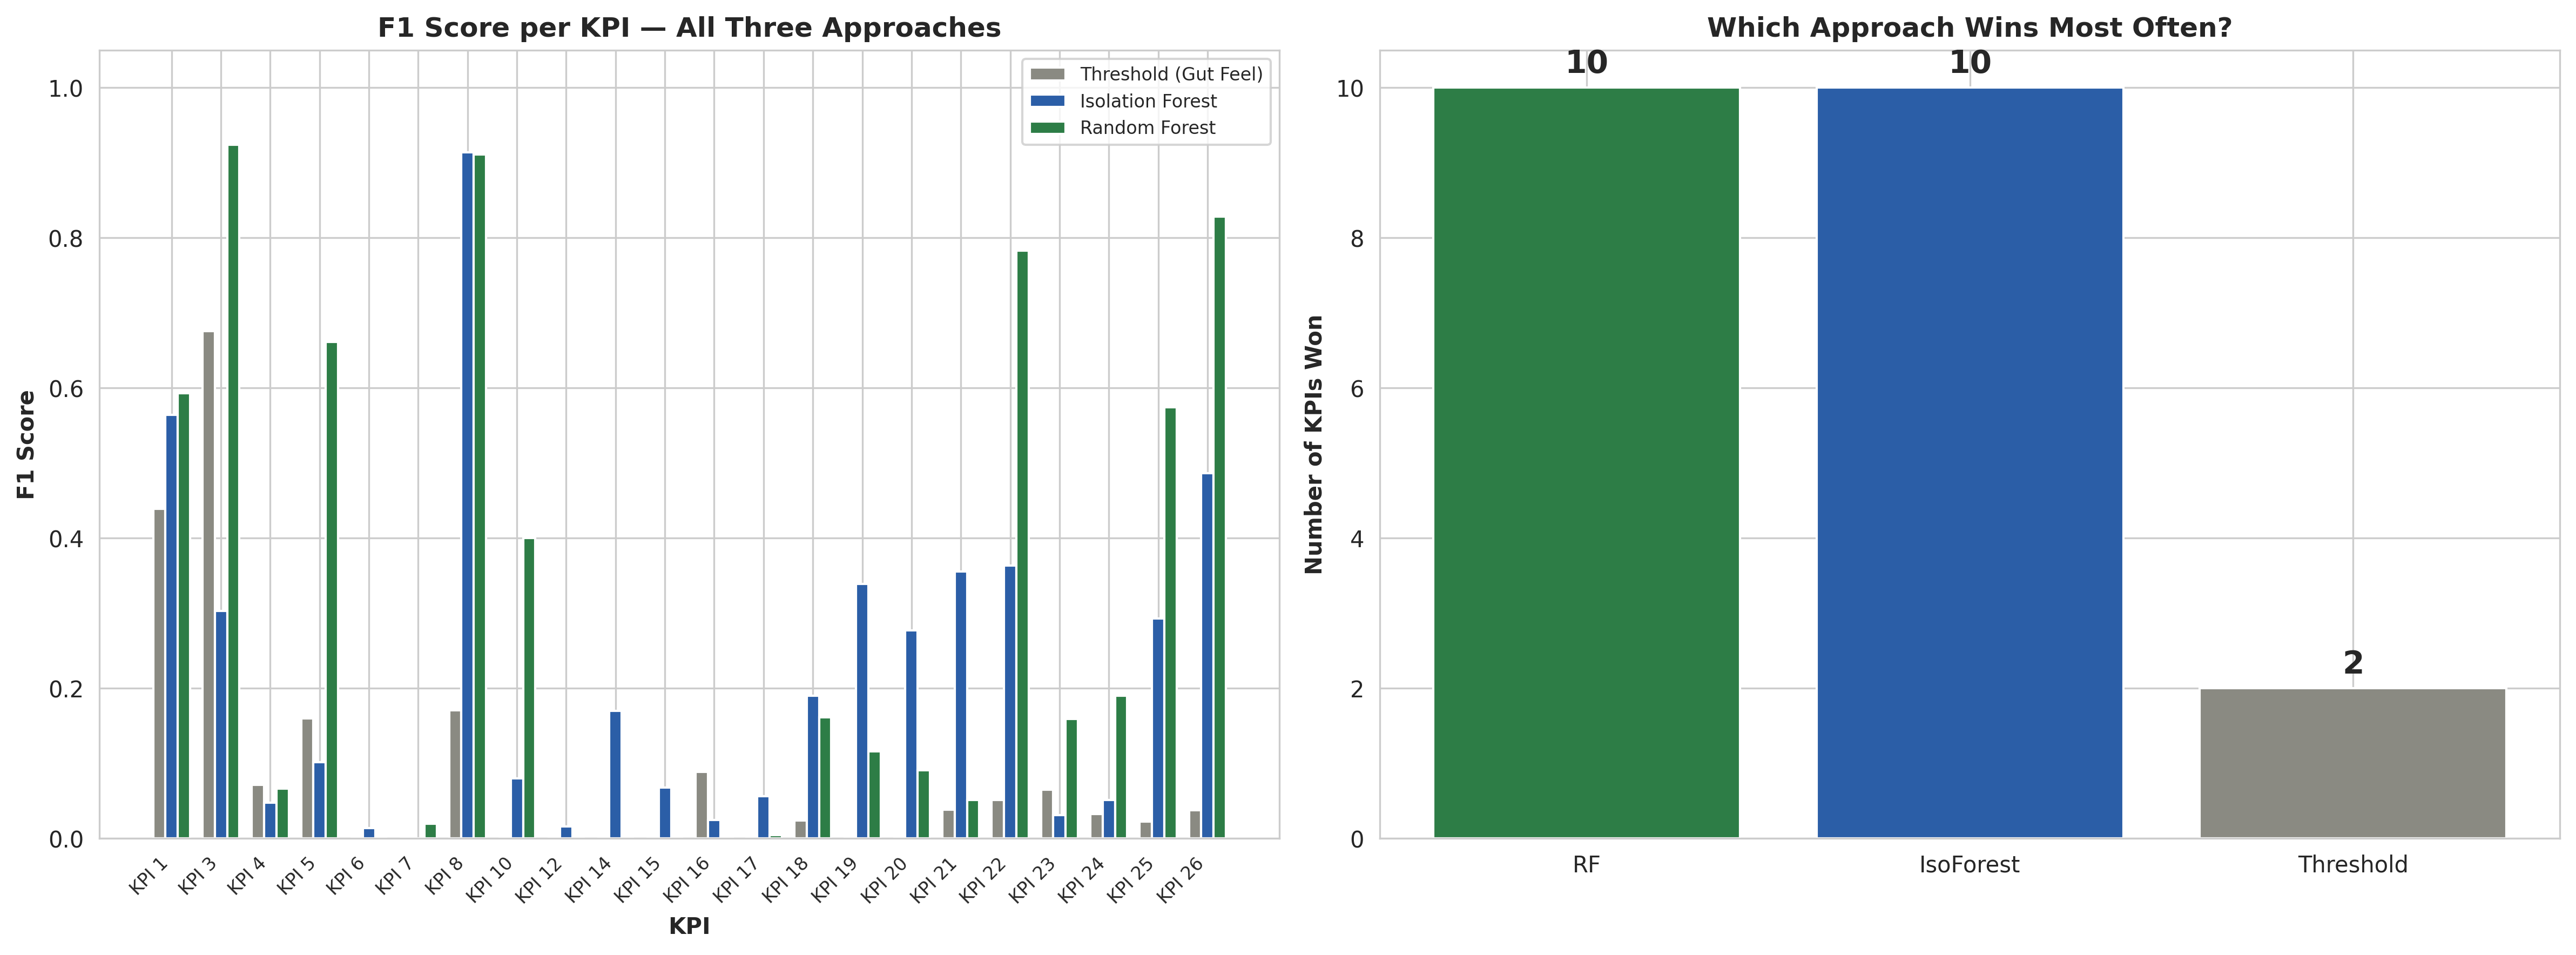
\includegraphics[width=\columnwidth]{fig02_per_kpi_comparison.png}
  \caption{Per-KPI model comparison. F1 scores for all three approaches across 22 evaluable KPIs (left) and win counts (right).}
  \label{fig:per_kpi}
\end{figure}

\subsection{Part A -- ML vs.\ Static Threshold}

\Cref{tab:perkpi} reports the per-KPI comparison.

\begin{table}[t]
  \centering
  \caption{Per-KPI best model selection -- ML vs.\ static threshold.}
  \label{tab:perkpi}
  \begin{tabular}{lrc}
    \toprule
    Method & KPIs won & Win rate \\
    \midrule
    Random Forest & 10 & 38.5\% \\
    Isolation Forest & 10 & 38.5\% \\
    Static threshold ($\mu \pm 3\sigma$) & 2 & 7.7\% \\
    Excluded (no anomalies in split) & 4 & 15.4\% \\
    \bottomrule
  \end{tabular}
\end{table}

Of the 22 evaluable KPIs, ML models won on 20 (91\%). However, win rate does not capture absolute performance: the mean per-KPI F1 was 0.41 and the median was 0.116, indicating that many KPIs remain difficult to detect even when ML outperforms the static threshold. The best performer (KPI~3) achieved F1\,=\,0.924, while most KPIs clustered at lower absolute performance.

\textbf{The tail where ML underperforms.} KPI~4 (anomaly rate 0.03\%) had too few positive examples for models to learn. KPI~16 (anomaly rate 6.15\%) saw all approaches perform poorly (best F1\,=\,0.089). These cases identify two boundary conditions: extremely sparse anomalies, and anomalies that do not manifest as statistical outliers in rolling-window features.

\begin{figure}[t]
  \centering
  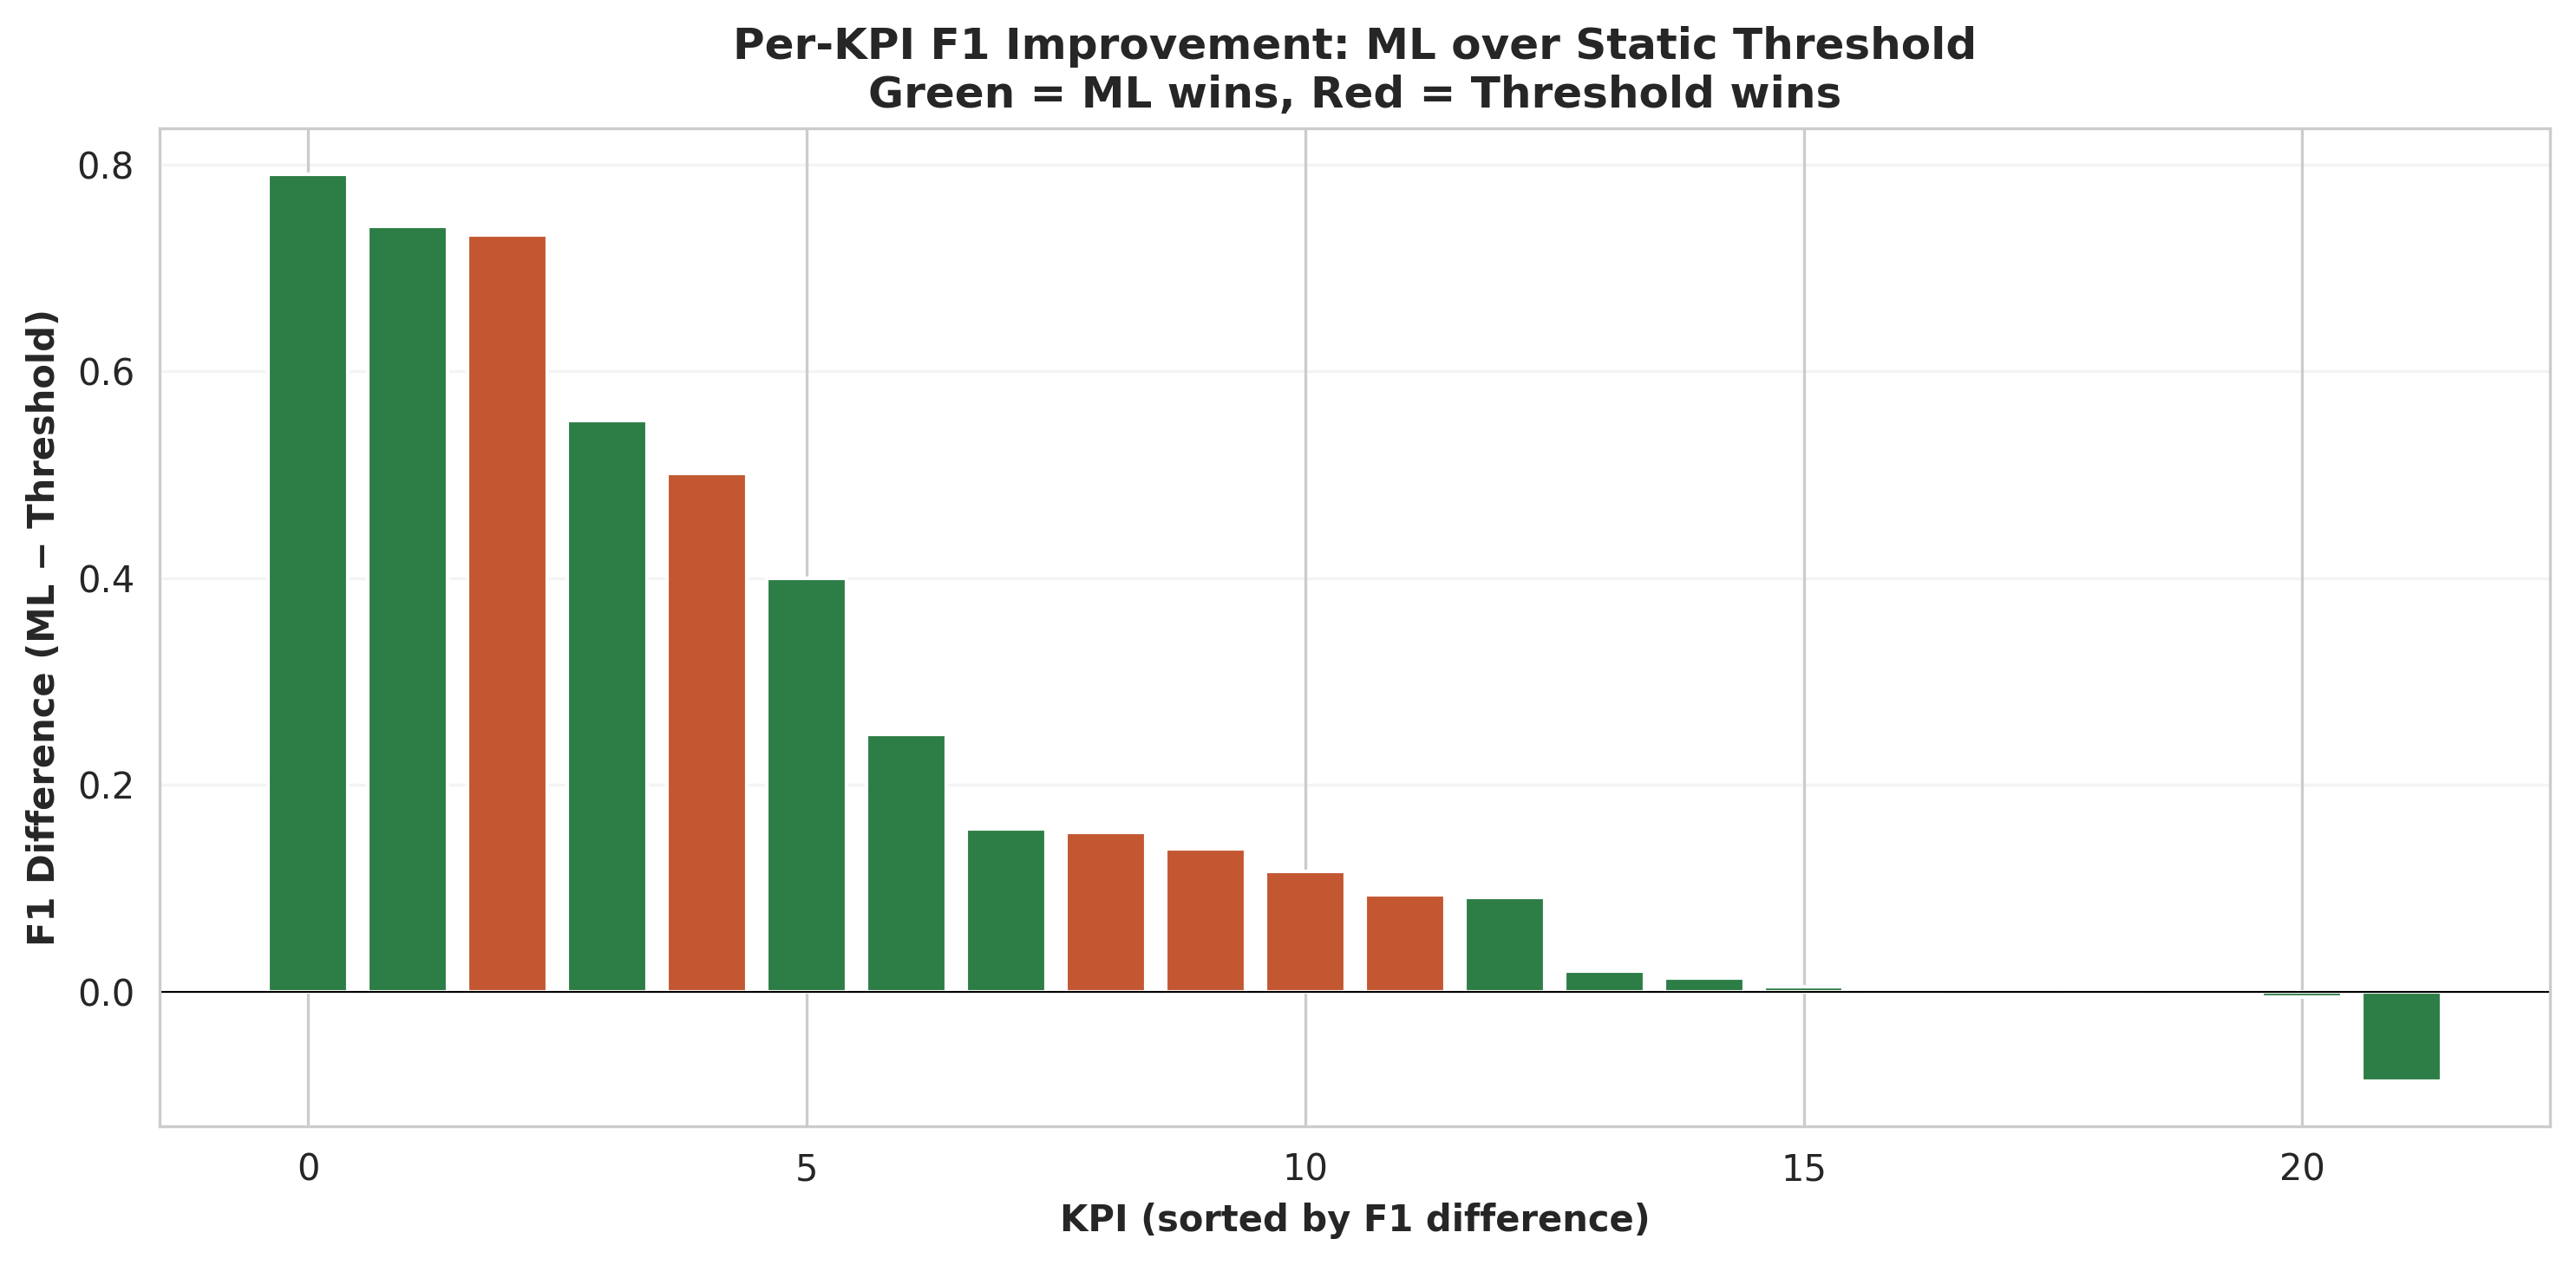
\includegraphics[width=\columnwidth]{fig03_f1_difference_distribution.png}
  \caption{Distribution of F1 differences (ML $-$ threshold) across evaluable KPIs.}
  \label{fig:f1_diff}
\end{figure}

\subsection{Part A -- Feature Waste}

\Cref{tab:ablation_a} reports the ablation study.

\begin{table}[t]
  \centering
  \caption{Ablation study -- effect of removing least-important features.}
  \label{tab:ablation_a}
  \begin{tabular}{rcrc}
    \toprule
    Retained & Removed (\%) & Mean F1 & $\Delta$ \\
    \midrule
    19 (all) & 0\% & 0.4065 & baseline \\
    15 & 21\% & 0.3989 & $-$0.008 \\
    12 & 37\% & 0.4066 & +0.000 \\
    \textbf{9} & \textbf{53\%} & \textbf{0.4142} & \textbf{+0.008} \\
    6 & 68\% & 0.3876 & $-$0.019 \\
    3 & 84\% & 0.3636 & $-$0.043 \\
    \bottomrule
  \end{tabular}
\end{table}

Removing 53\% of features \emph{improved} mean F1 from 0.4065 to 0.4142. Performance degraded meaningfully only below 9 features.

\begin{figure}[t]
  \centering
  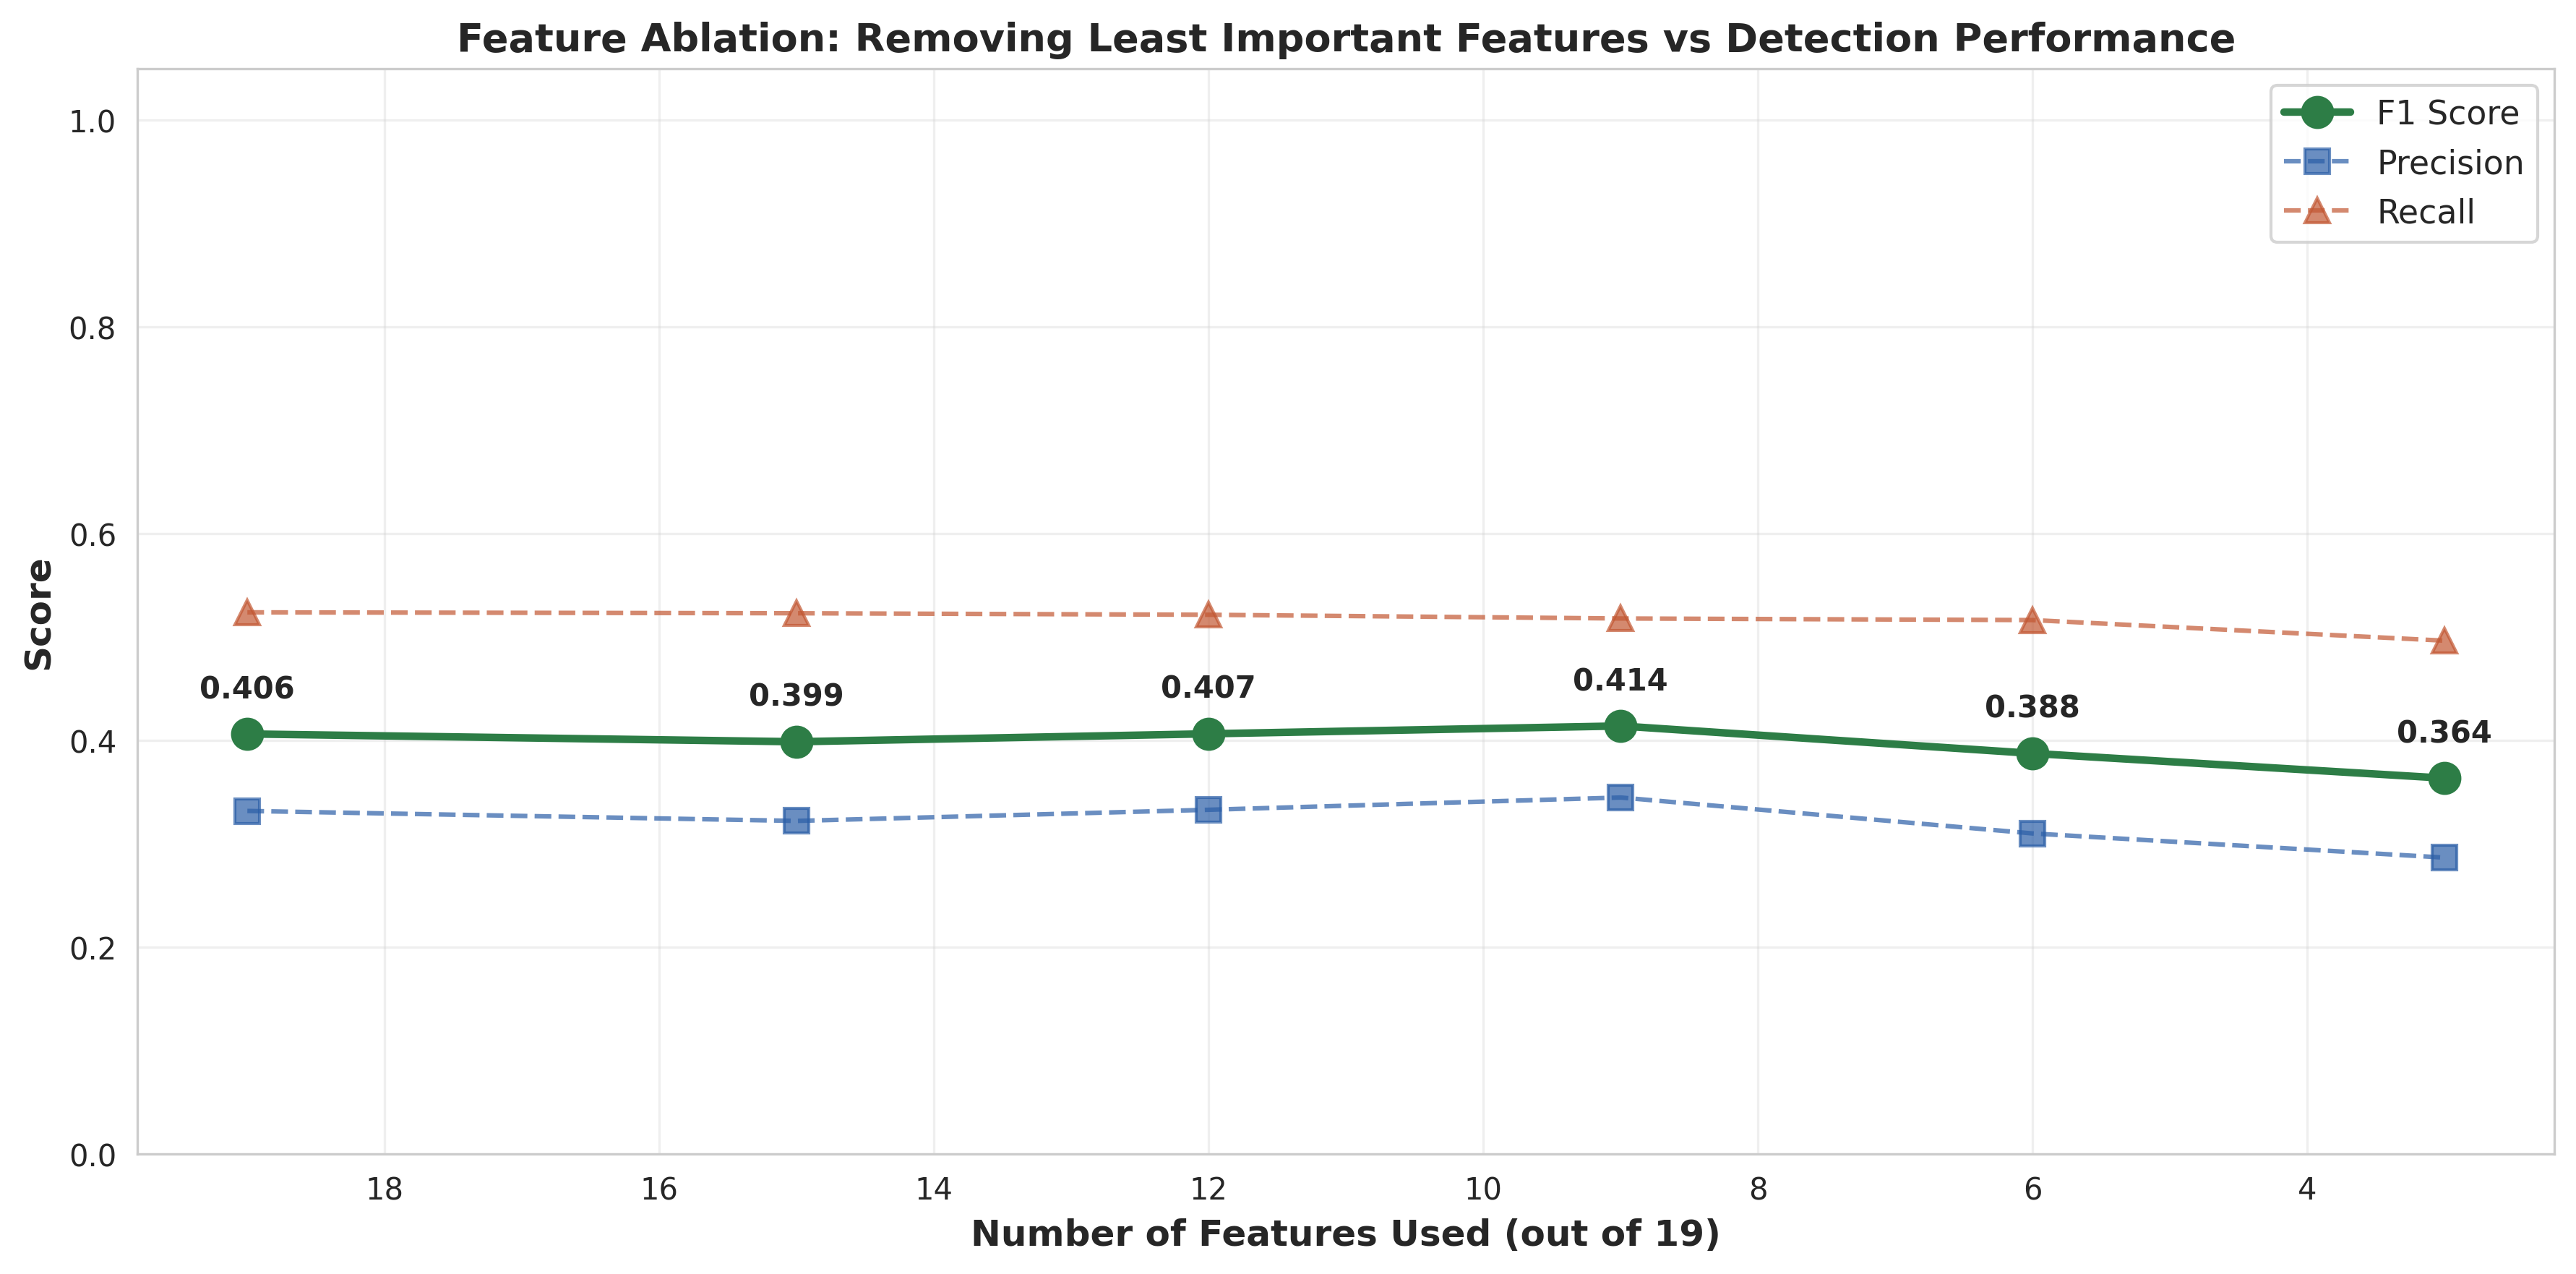
\includegraphics[width=\columnwidth]{fig04_ablation_curve.png}
  \caption{Ablation curve. Mean F1 vs.\ number of features removed.}
  \label{fig:ablation_curve}
\end{figure}

\subsection{Part A -- SHAP: Feature Importance Varies Across KPIs}

SHAP analysis revealed that \texttt{rolling\_min\_15} ranked first for all three representative KPIs, but the remaining feature rankings differed substantially. A heatmap of feature importances across all 22 evaluable KPIs confirmed this: no single feature ranked in the top 3 for every KPI (\Cref{fig:shap,fig:heatmap}).

\begin{figure}[t]
  \centering
  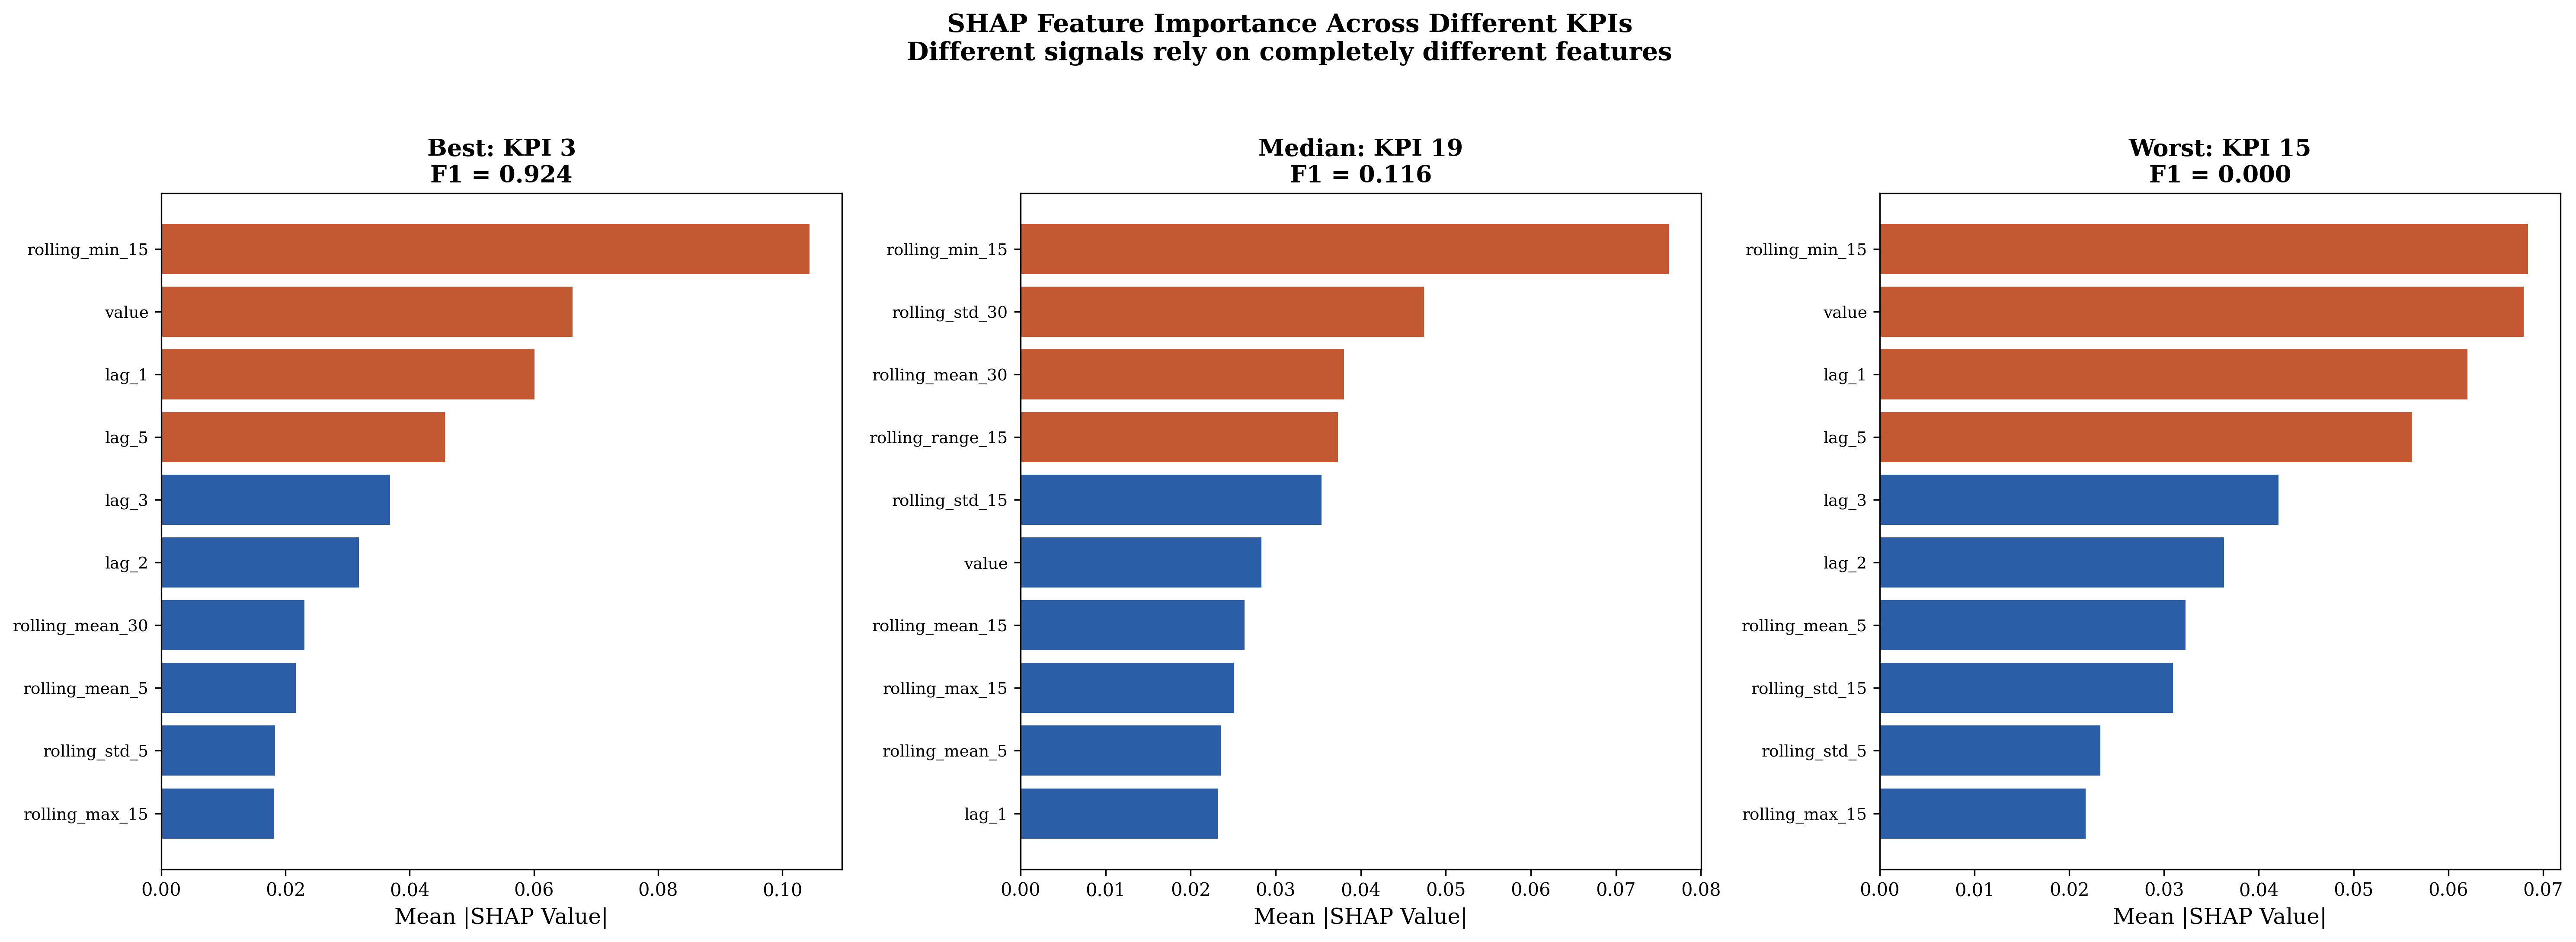
\includegraphics[width=\columnwidth]{fig05_shap_beeswarm.png}
  \caption{SHAP beeswarm plots for 3 representative KPIs.}
  \label{fig:shap}
\end{figure}

\begin{figure}[t]
  \centering
  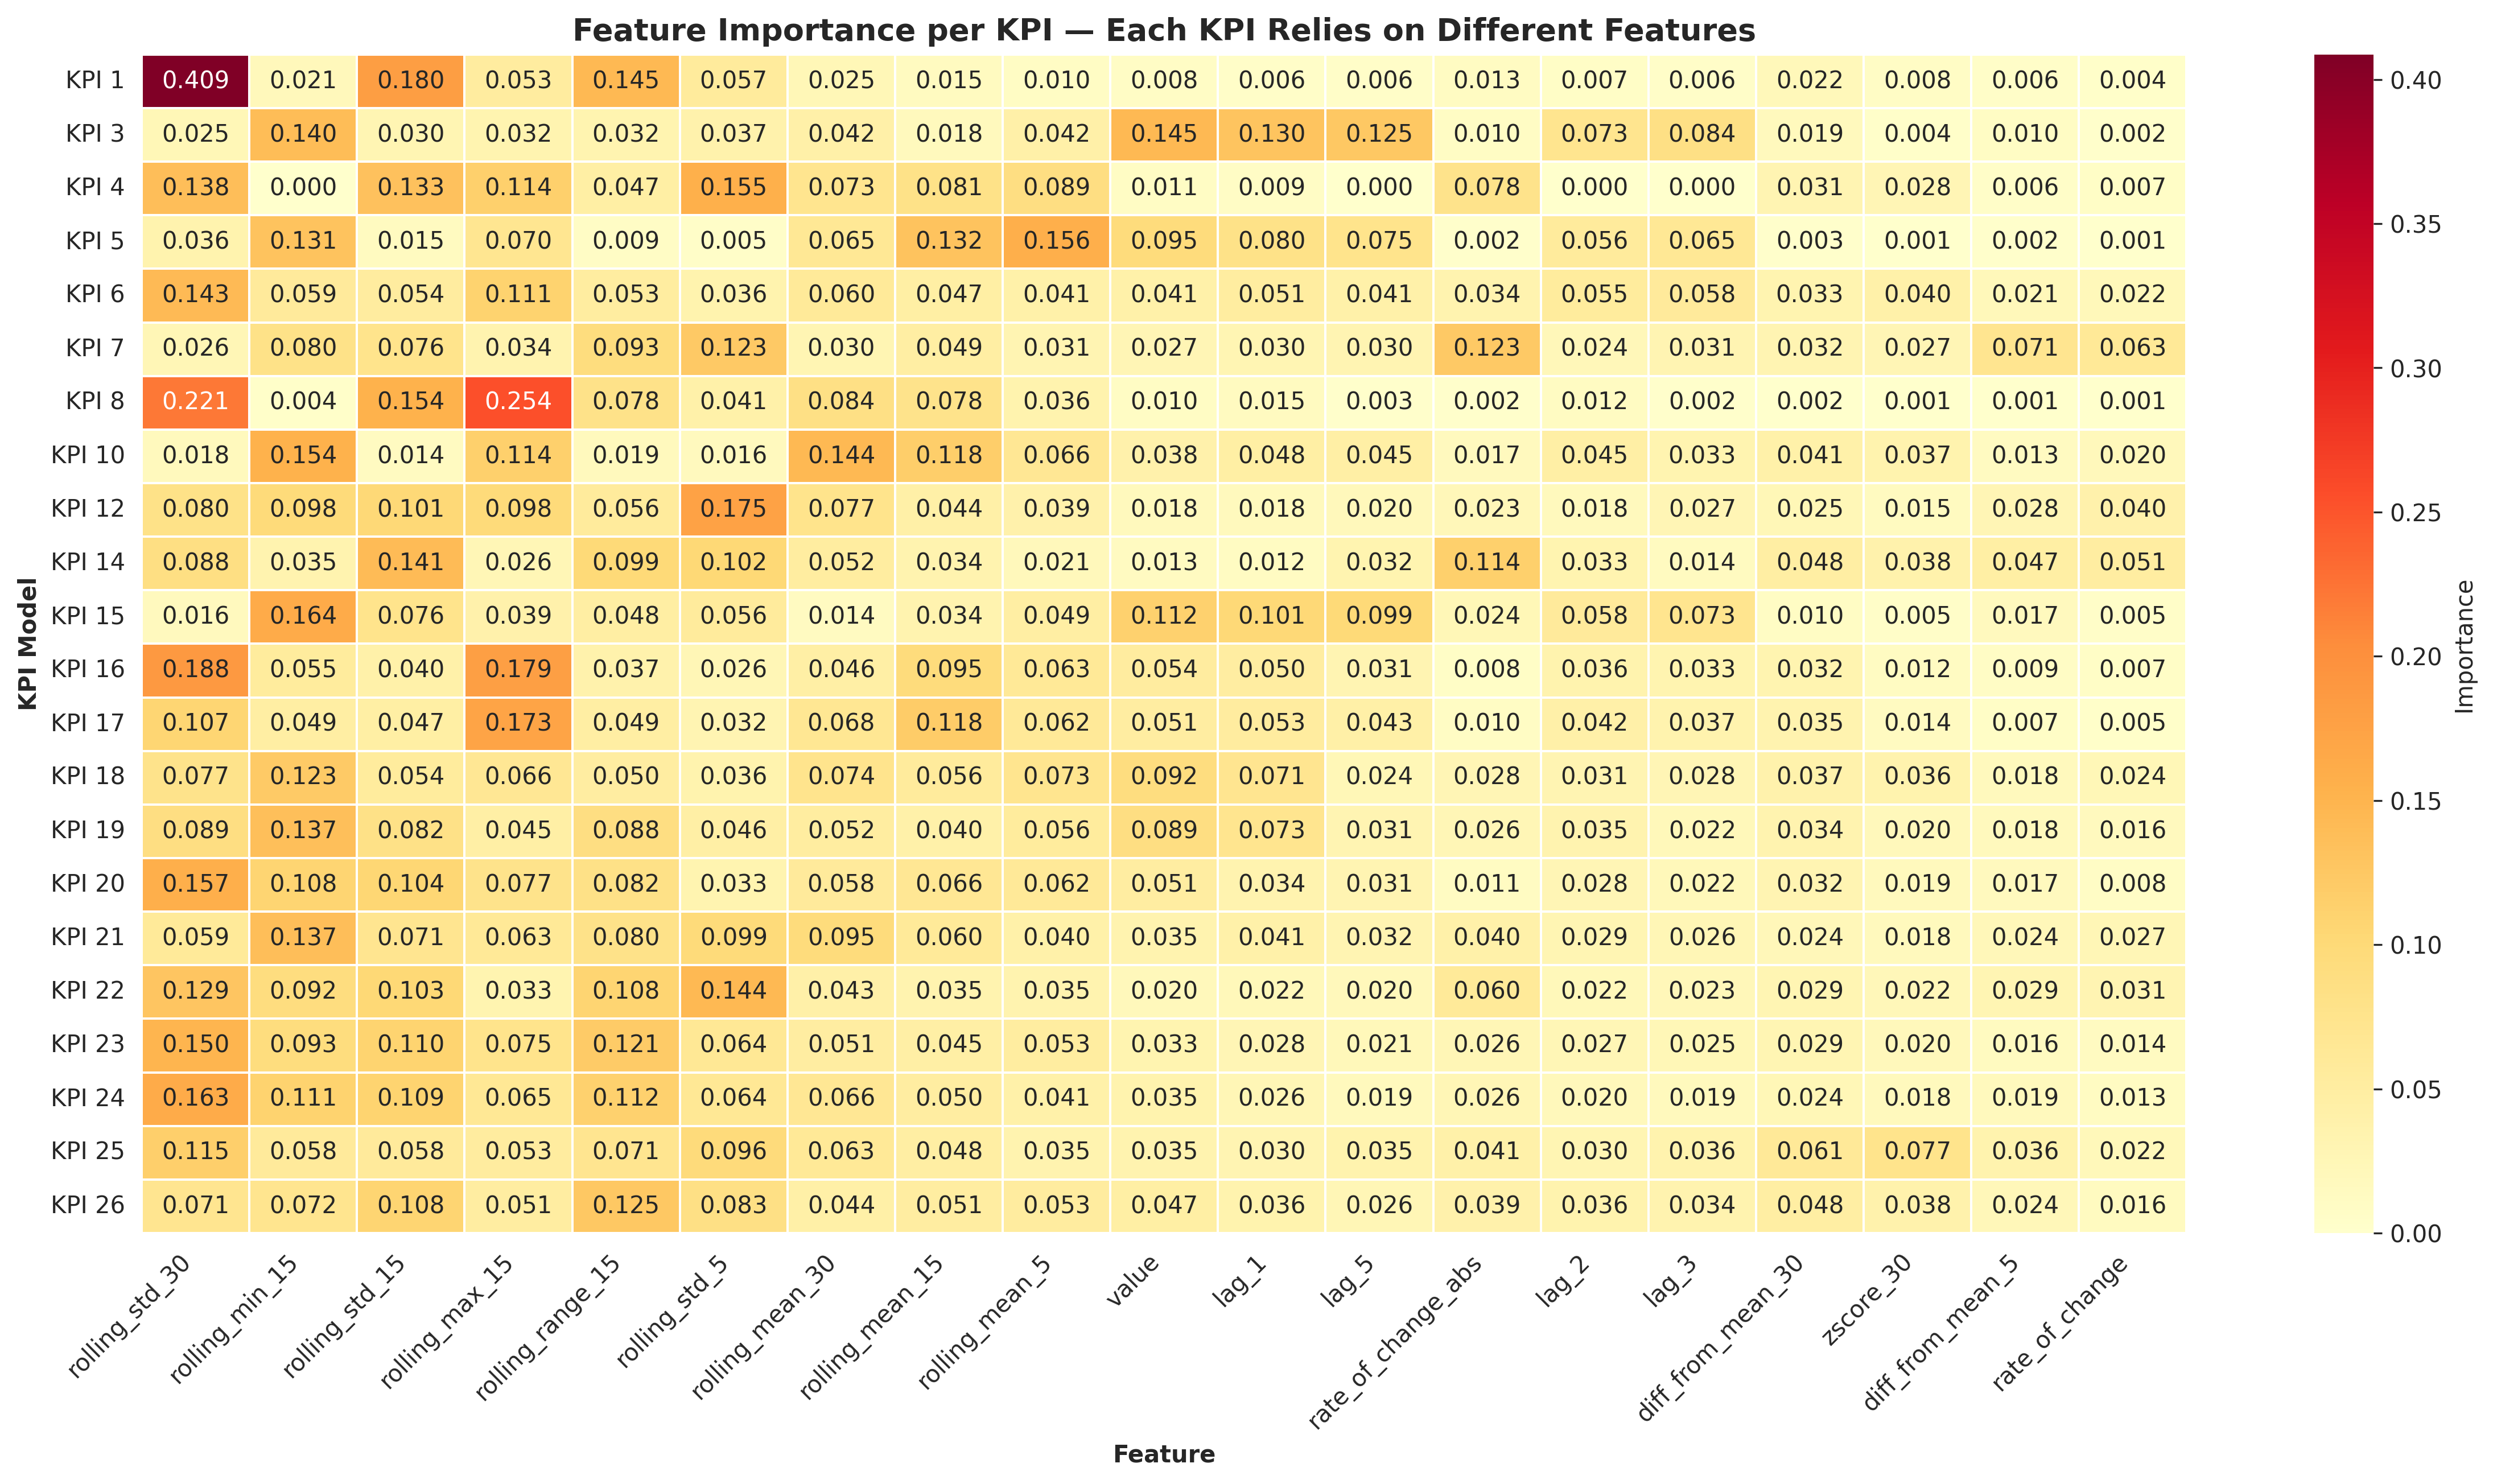
\includegraphics[width=\columnwidth]{fig_supp_feature_heatmap.png}
  \caption{Feature importance heatmap across all evaluable KPIs.}
  \label{fig:heatmap}
\end{figure}

\subsection{Part B -- Log-Level Classification}

\Cref{tab:classification} reports the 5-fold stratified cross-validation results.

\begin{table}[t]
  \centering
  \caption{Log-level prediction -- model comparison (5-fold stratified CV).}
  \label{tab:classification}
  \begin{tabular}{llcc}
    \toprule
    Model & Type & Accuracy & Macro F1 \\
    \midrule
    Random guess & Baseline & 0.319 & 0.251 \\
    Keyword heuristic & Heuristic & 0.607 & 0.377 \\
    Logistic Regression & ML & 0.646\tiny{$\pm$0.018} & 0.591\tiny{$\pm$0.028} \\
    Random Forest & ML & 0.958\tiny{$\pm$0.004} & 0.953\tiny{$\pm$0.005} \\
    XGBoost & ML & 0.967\tiny{$\pm$0.003} & 0.961\tiny{$\pm$0.003} \\
    \bottomrule
  \end{tabular}
\end{table}

XGBoost achieved macro F1 of 0.961, substantially outperforming the keyword heuristic (0.377). The confusion matrix (\Cref{fig:confusion}) shows near-uniform accuracy across all four classes: DEBUG 96.3\%, ERROR 94.7\%, INFO 97.9\%, WARN 96.4\%.

\begin{figure}[t]
  \centering
  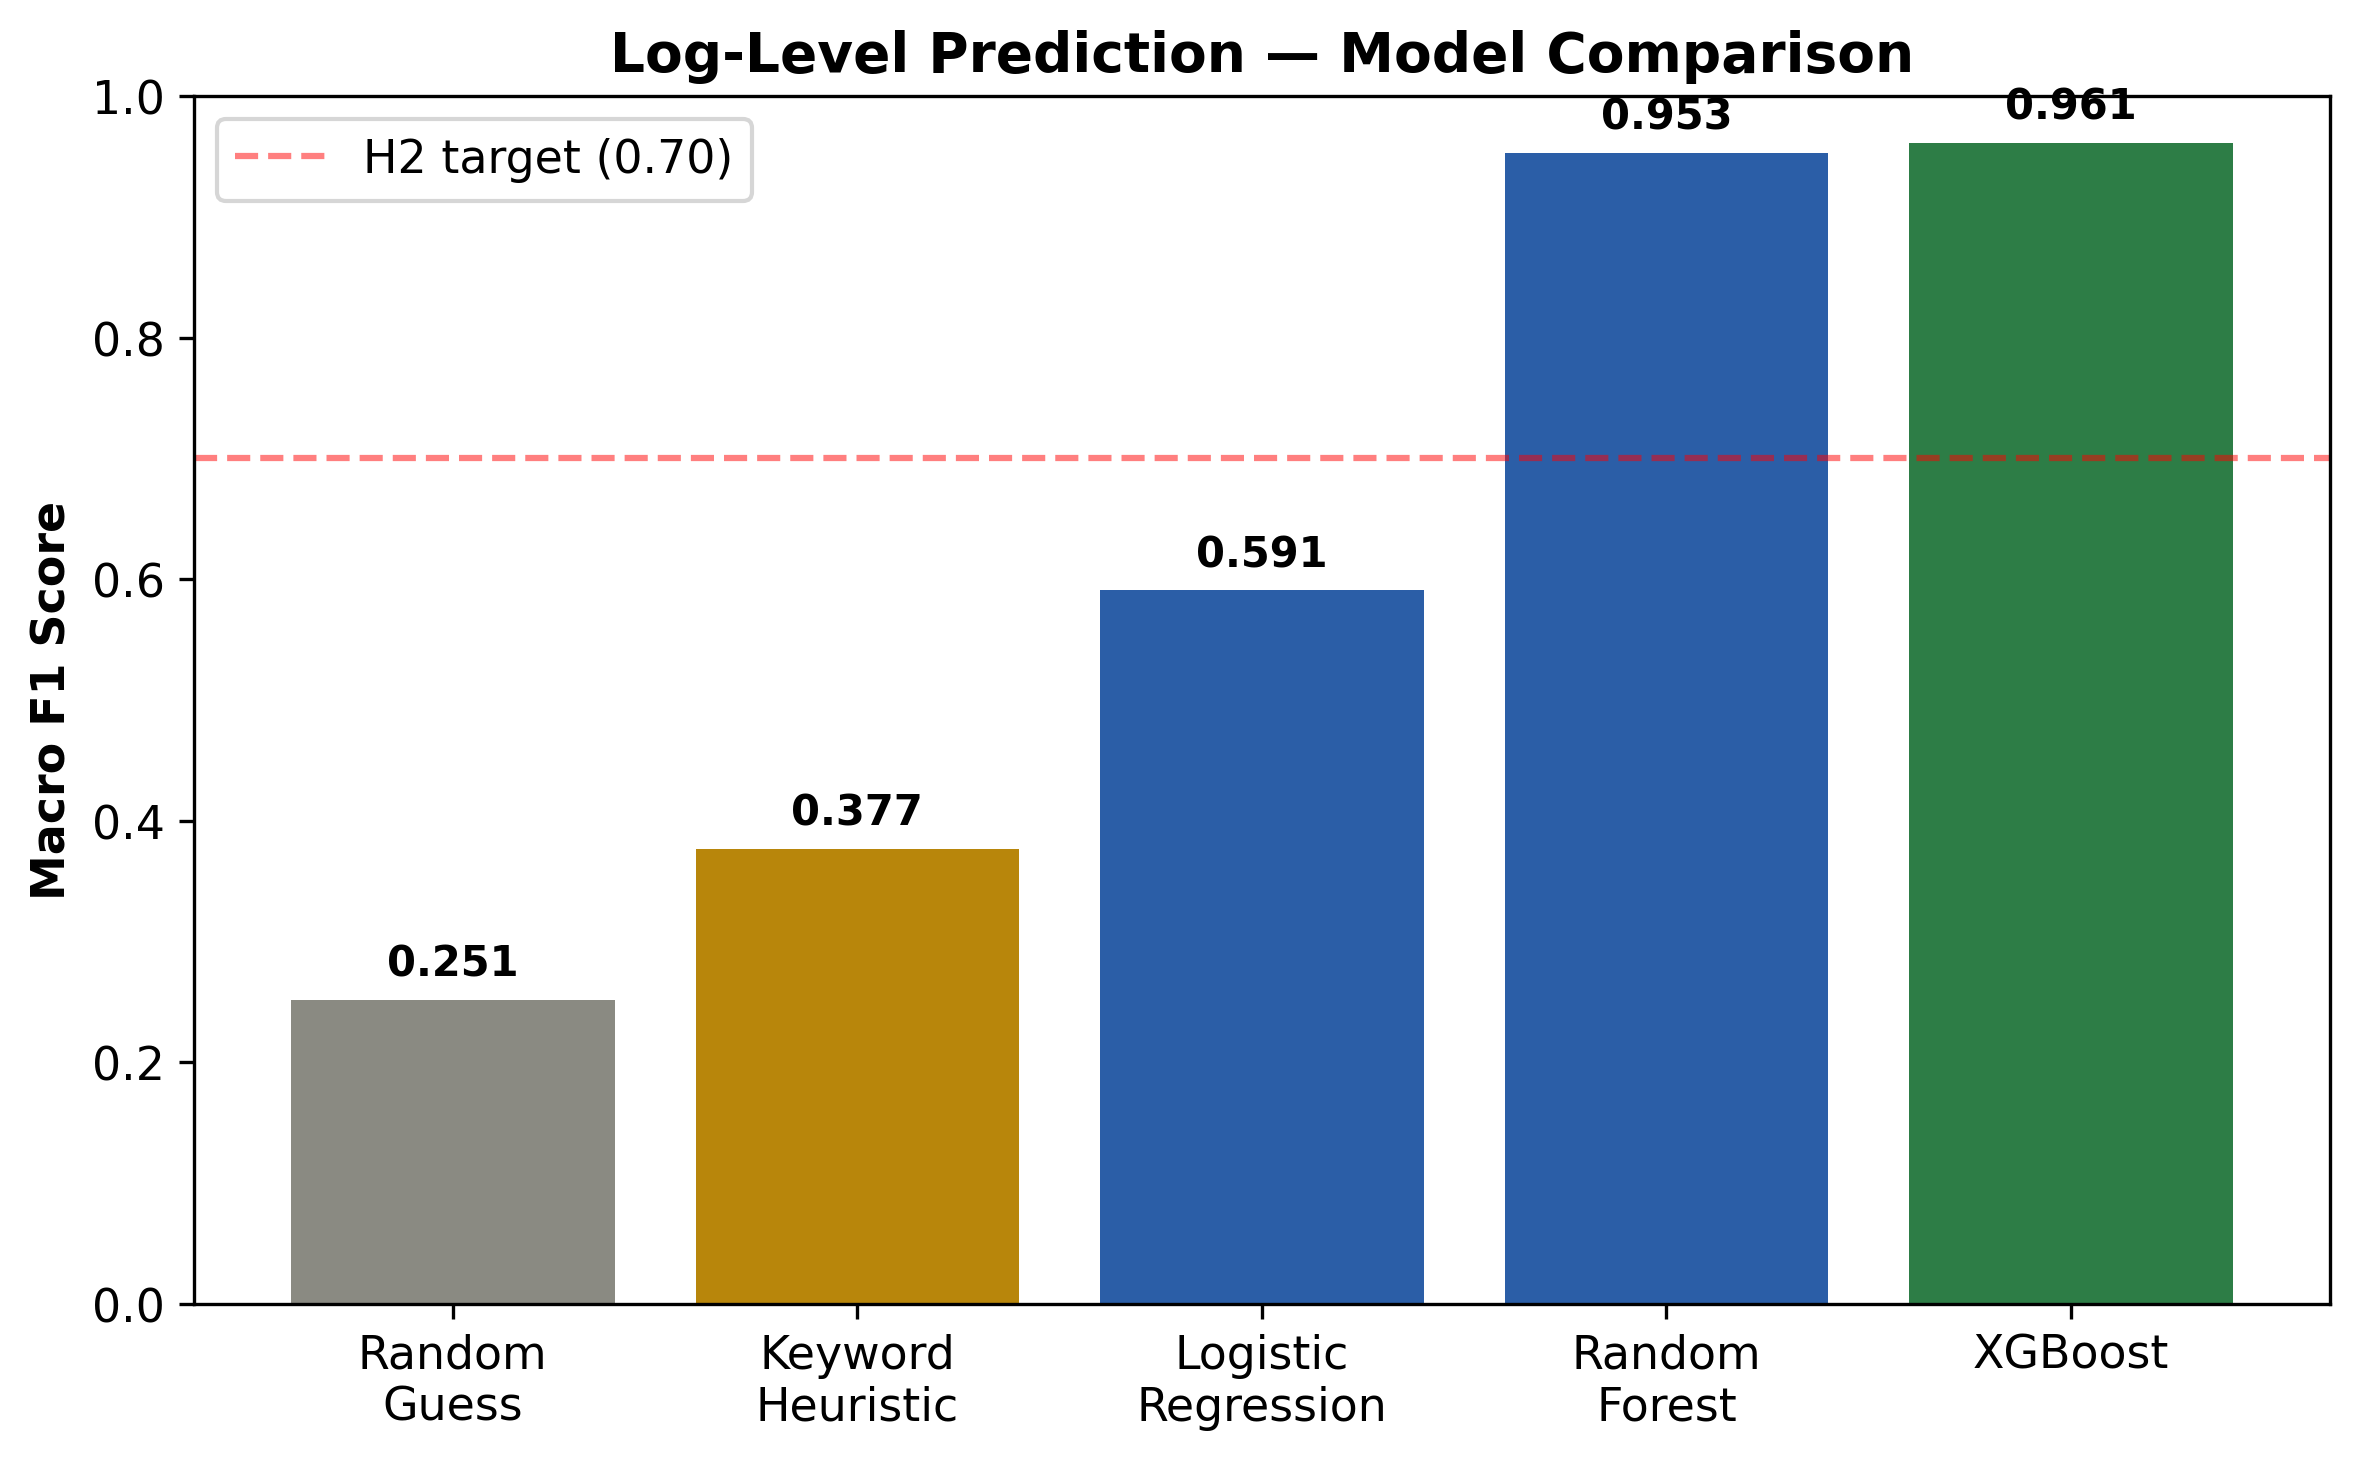
\includegraphics[width=\columnwidth]{fig07_model_comparison.png}
  \caption{Log-level prediction model comparison.}
  \label{fig:model_comparison}
\end{figure}

\begin{figure}[t]
  \centering
  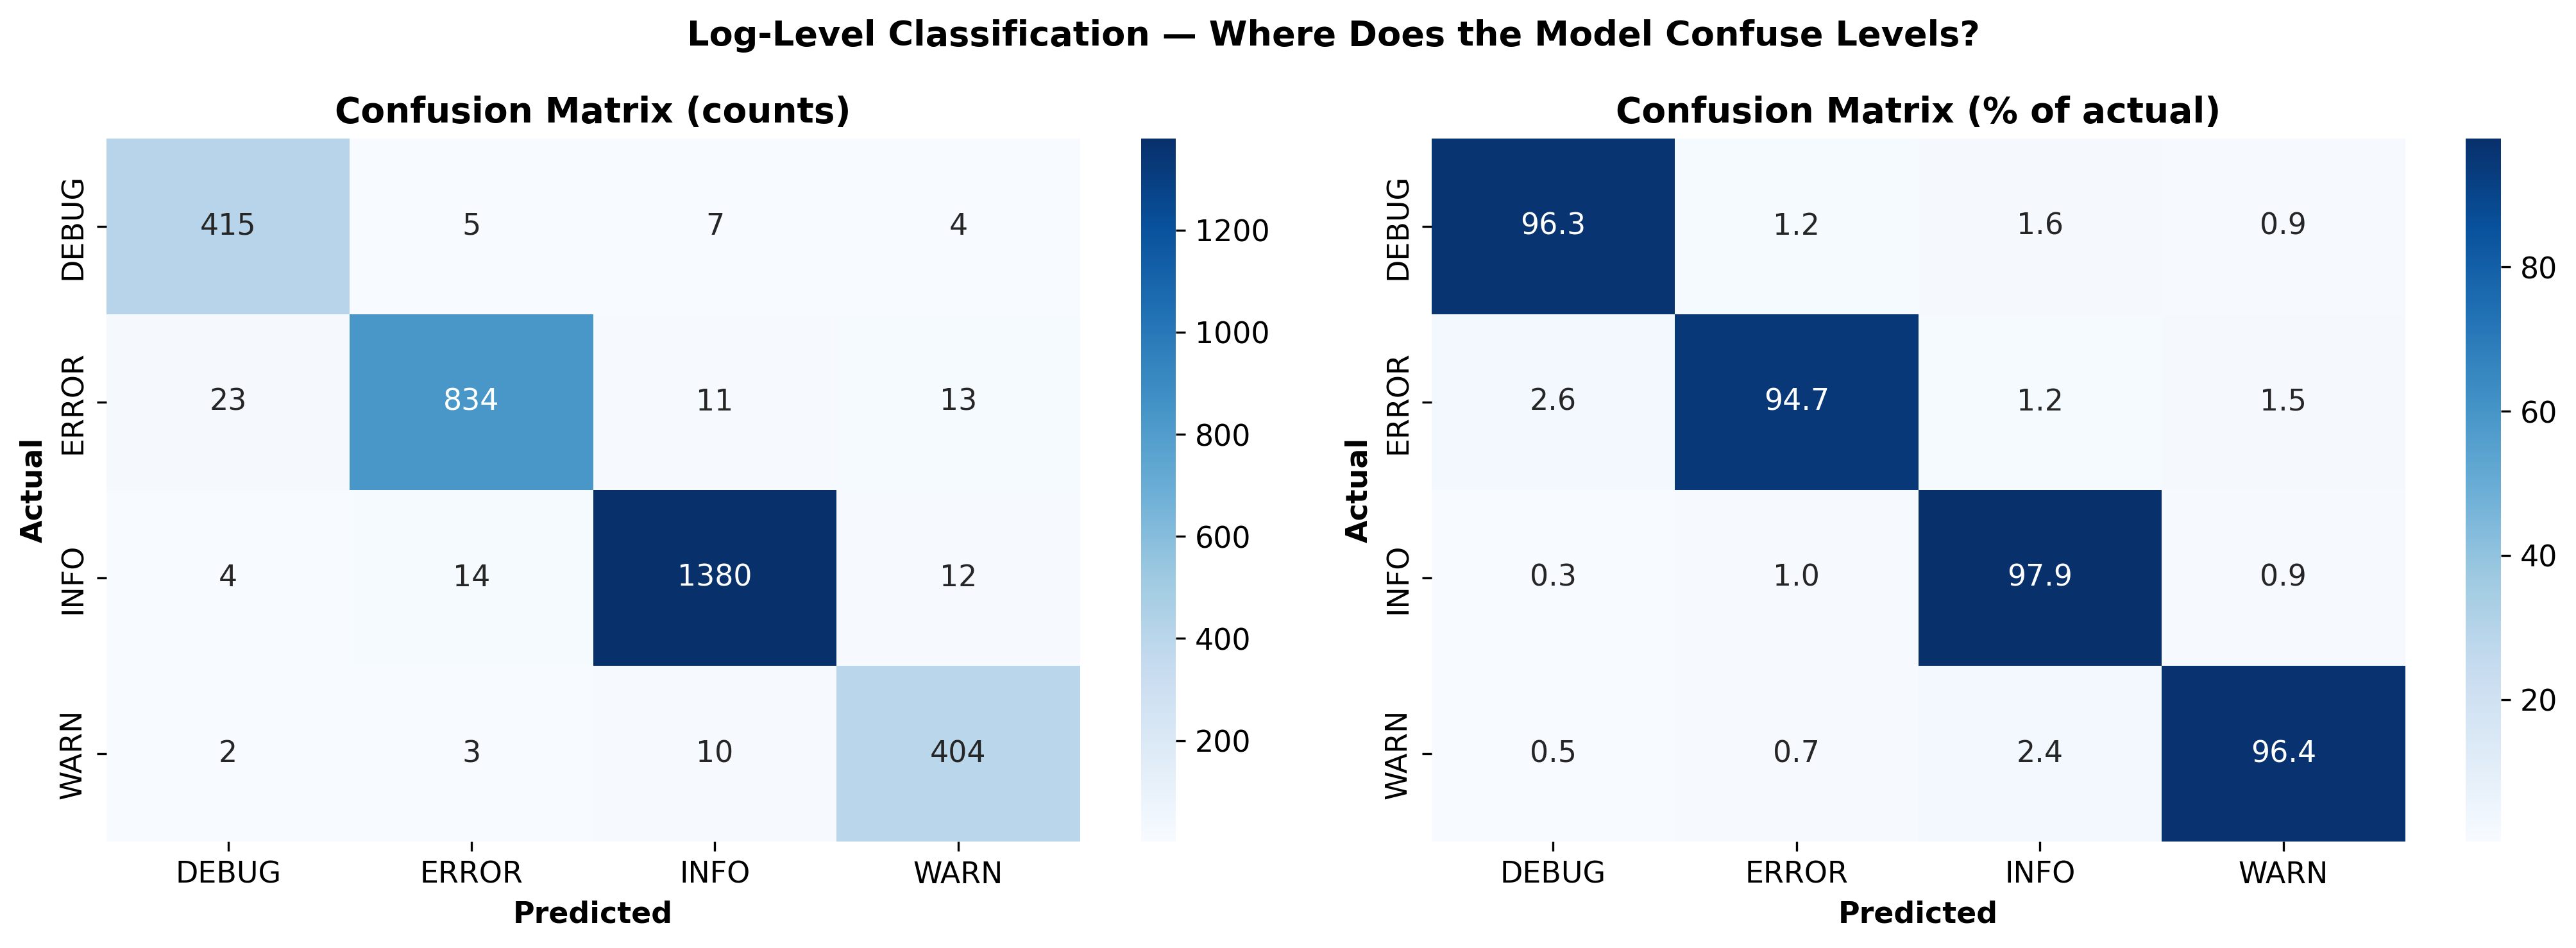
\includegraphics[width=\columnwidth]{fig08_confusion_matrix.png}
  \caption{Confusion matrix (percentage) for XGBoost classifier.}
  \label{fig:confusion}
\end{figure}

\subsection{Part B -- Feature Ablation}

\Cref{tab:ablation_b} reports the feature ablation results.

\begin{table}[t]
  \centering
  \caption{Feature ablation -- macro F1 under each condition.}
  \label{tab:ablation_b}
  \begin{tabular}{lrcc}
    \toprule
    Condition & Feat. & CV F1 & CP F1 \\
    \midrule
    Full (all features) & 715 & 0.965 & 0.928 \\
    \textbf{No message TF-IDF} & \textbf{515} & \textbf{0.958} & \textbf{0.921} \\
    No level names & 459 & 0.710 & 0.519 \\
    Context TF-IDF only & 500 & 0.936 & 0.907 \\
    Structural + file type & 15 & 0.634 & 0.460 \\
    Message TF-IDF only & 200 & 0.504 & 0.382 \\
    Keyword heuristic & 6 & 0.378 & 0.382 \\
    \bottomrule
  \end{tabular}
\end{table}

Four key observations. First, removing message TF-IDF reduces cross-project F1 by only 0.006 (from 0.928 to 0.921). Second, message TF-IDF alone (0.382) performs no better than the keyword heuristic (0.382). Third, no level depends on message text. Fourth, and most critically, stripping level-name tokens collapses cross-project F1 from 0.921 to 0.519 -- only modestly above the structural-only baseline (0.460). The model primarily predicts log level from the levels of \emph{neighbouring log statements} in the $\pm$5-line window.

We adopt the ``no message'' model (macro F1\,=\,0.921 cross-project) as the primary result, but qualify the interpretation: the context signal is dominated by neighbouring log-level tokens rather than broader code patterns (\Cref{sec:clustering}).

\begin{figure}[t]
  \centering
  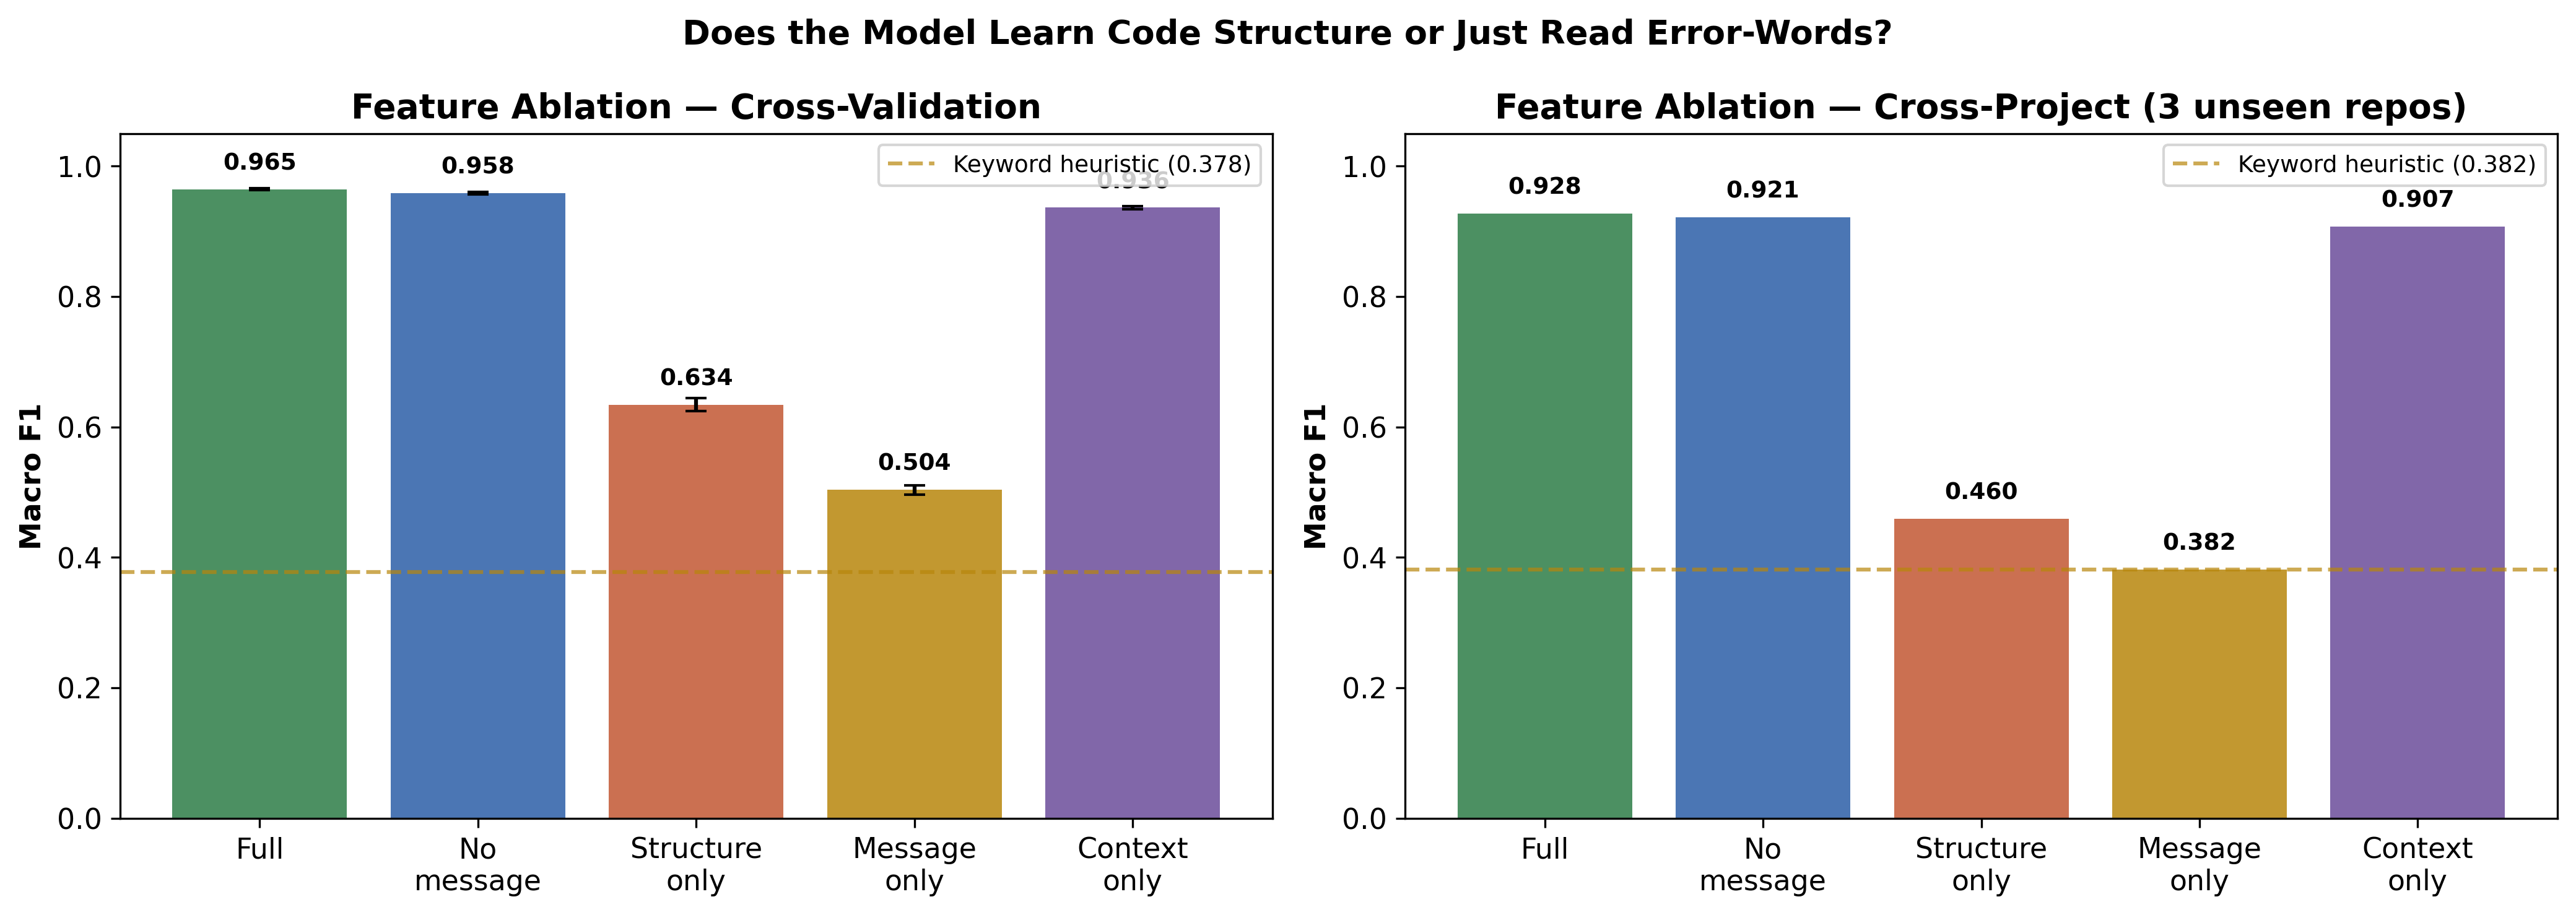
\includegraphics[width=\columnwidth]{fig09_ablation_bar.png}
  \caption{Feature ablation. Macro F1 under each condition.}
  \label{fig:ablation_bar}
\end{figure}

\subsection{Part B -- Cross-Project Generalisation}

\Cref{tab:crossproject} reports the cross-project evaluation on three unseen repositories.

\begin{table}[t]
  \centering
  \caption{Cross-project evaluation -- ``no message'' model vs.\ keyword heuristic on unseen repos.}
  \label{tab:crossproject}
  \begin{tabular}{llrccc}
    \toprule
    Repo & Domain & $n$ & Heur. & XGB & Impr. \\
    \midrule
    Strapi & CMS & 1,063 & .372 & .907 & +144\% \\
    Immich & Photos & 570 & .374 & .906 & +142\% \\
    Cal.com & Sched. & 1,822 & .379 & .929 & +145\% \\
    \midrule
    \textbf{Full ctx.} & -- & \textbf{3,455} & \textbf{.382} & \textbf{.921} & \textbf{+141\%} \\
    \textbf{No levels} & -- & \textbf{3,455} & \textbf{.382} & \textbf{.519} & \textbf{+36\%} \\
    \bottomrule
  \end{tabular}
\end{table}

``Full context'' includes neighbouring log-level tokens (the realistic deployment scenario). ``No level names'' approximates a greenfield scenario. Both numbers are true; the deployment context determines which applies.

\begin{figure}[t]
  \centering
  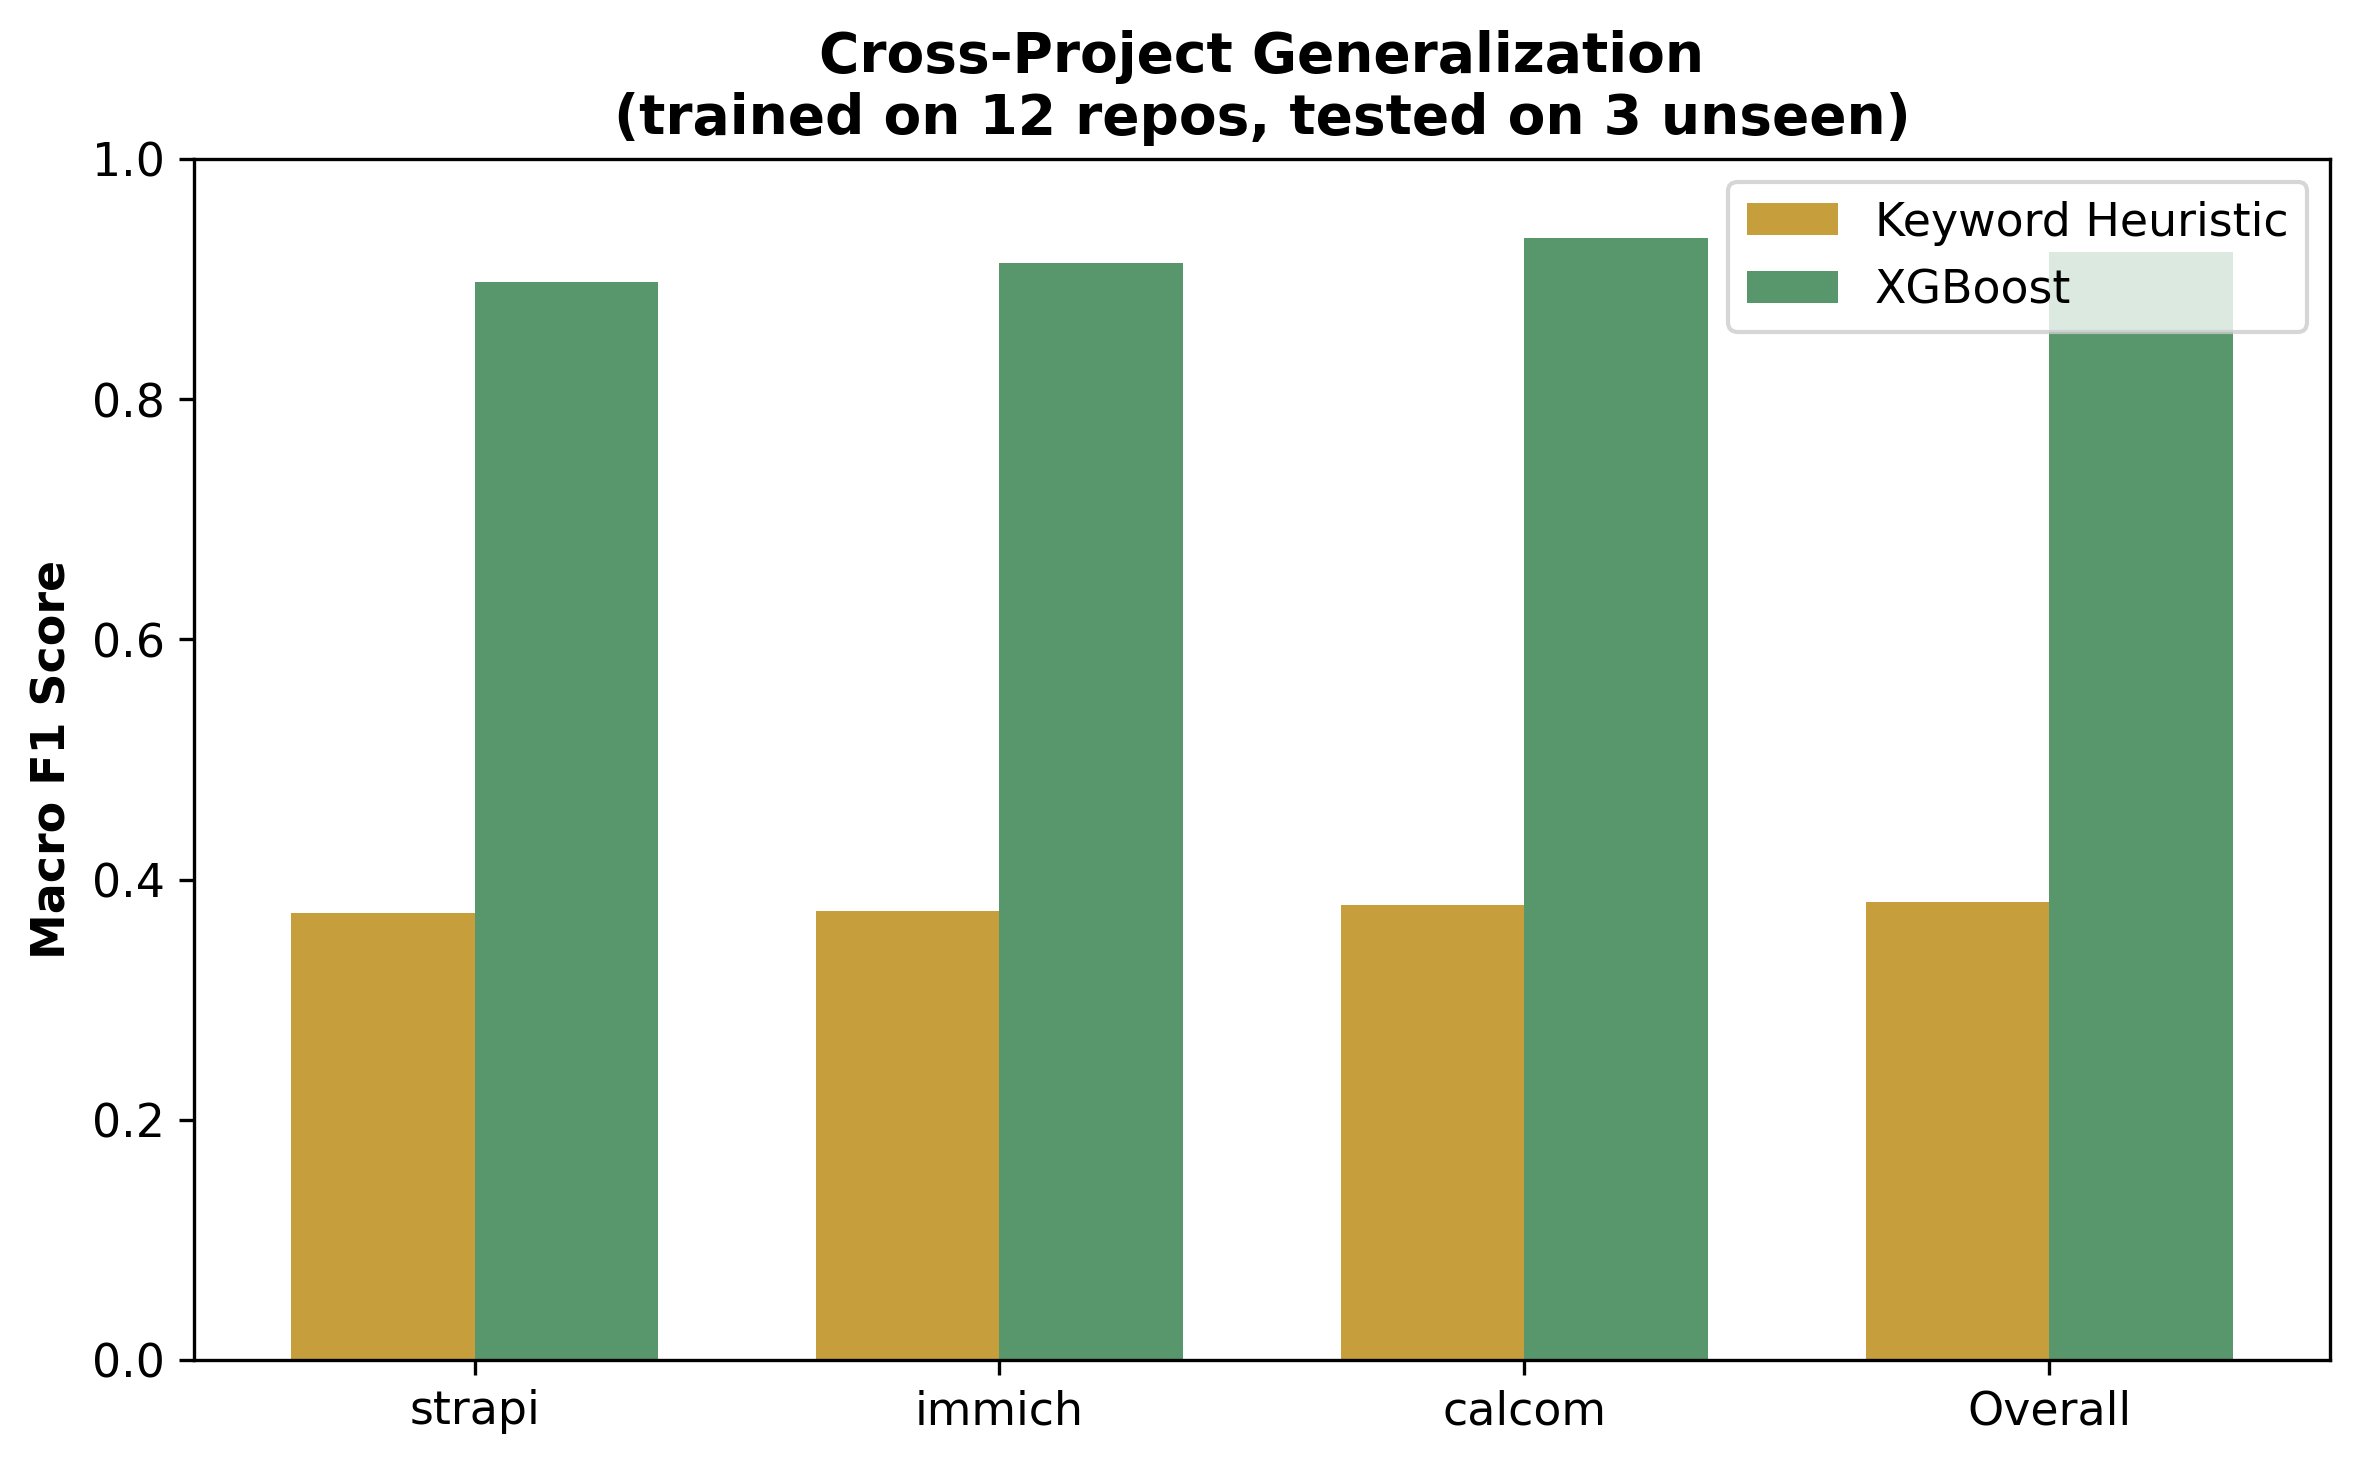
\includegraphics[width=\columnwidth]{fig10_cross_project.png}
  \caption{Cross-project generalisation. Heuristic vs.\ XGBoost.}
  \label{fig:crossproject}
\end{figure}

\subsection{Part B -- Feature Importance}

The top 5 features are all code-context terms: \texttt{ctx:warn} (0.114), \texttt{ctx:debug} (0.100), \texttt{ctx:console\_log} (0.066), \texttt{ctx:logger\_warn} (0.060), and \texttt{ctx:logger\_debug} (0.056). These are level names of neighbouring log statements captured in the $\pm$5-line context window. The level-name-stripped ablation confirms this is the dominant signal.

\begin{figure}[t]
  \centering
  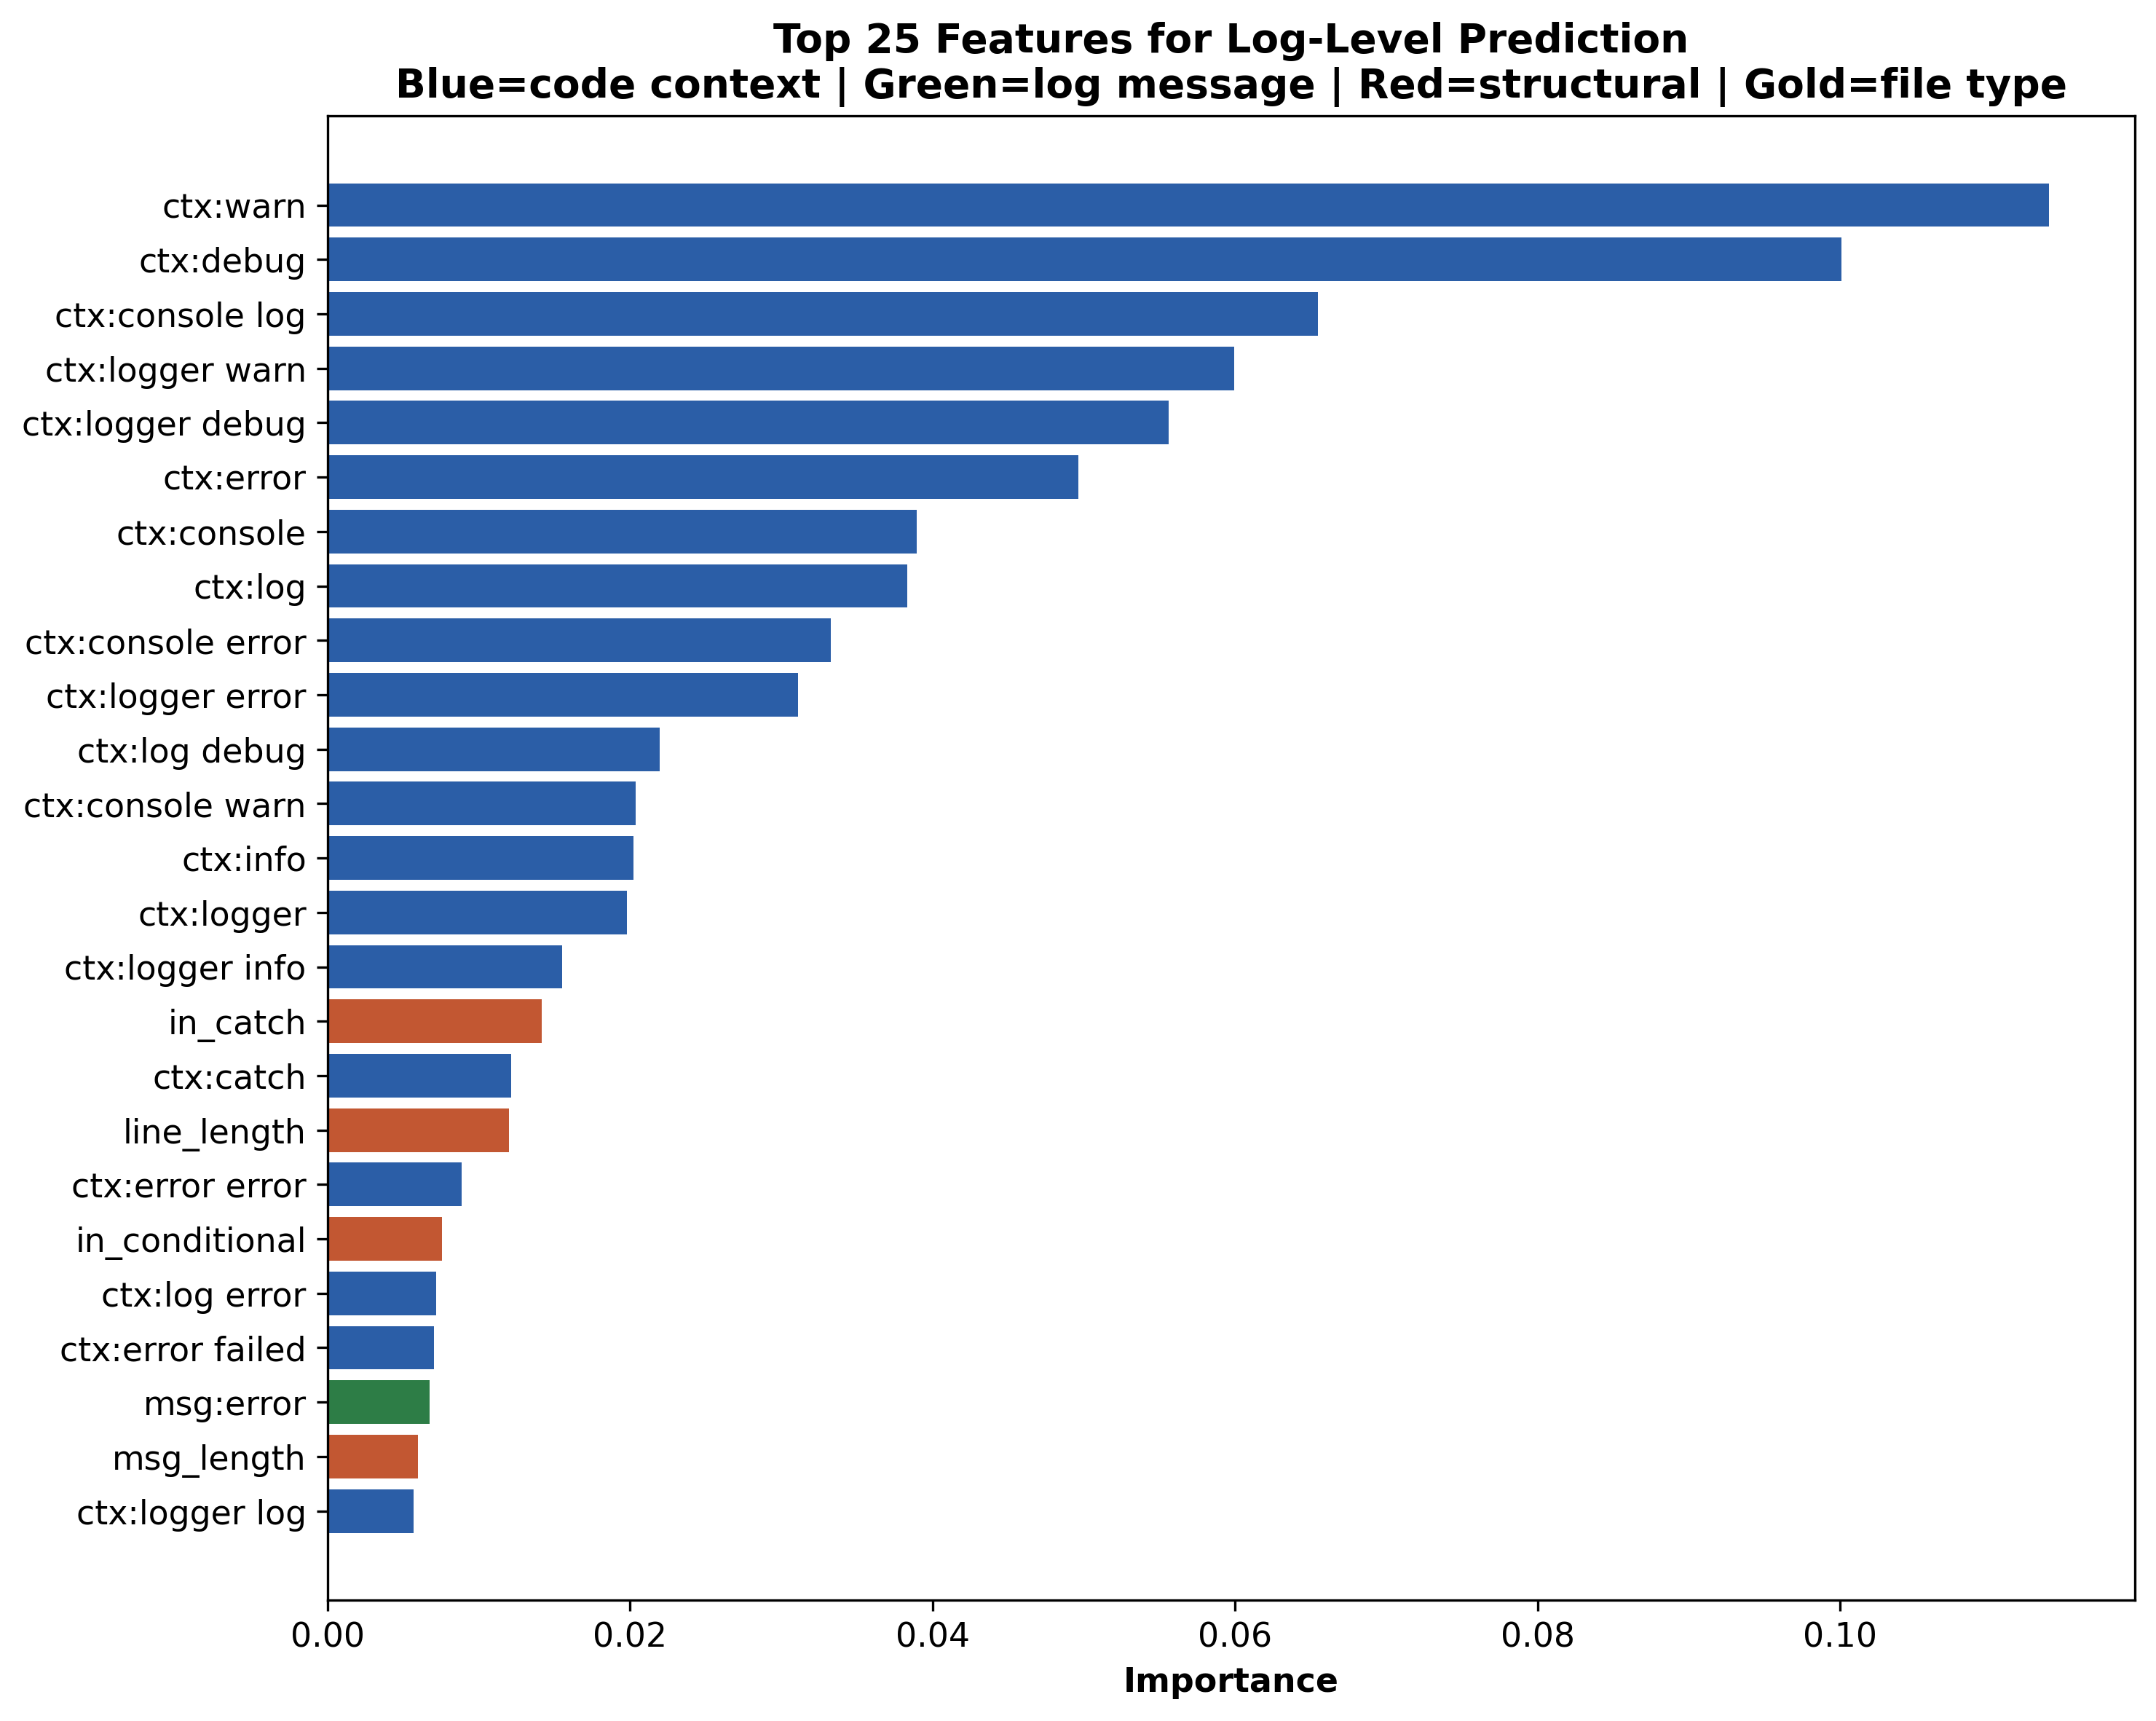
\includegraphics[width=\columnwidth]{fig11_feature_importance.png}
  \caption{Top 25 features for log-level prediction.}
  \label{fig:feature_importance}
\end{figure}

\subsection{Part B -- Inconsistency Analysis}

Error analysis identified cases where the model's prediction and the developer's label conflict. Examples include a \texttt{catch}-block log labelled DEBUG by the developer but predicted ERROR by the model (Strapi), and an INFO-level log inside a \texttt{catch} block predicted as ERROR (Supabase). These cases illustrate that individual developer choices sometimes deviate from corpus-wide norms.

% ===========================================================================
% 5. DISCUSSION
% ===========================================================================
\section{Discussion}
\label{sec:discussion}

\subsection{What Learned Models Outperform -- and What They Do Not}

Learned models substantially outperform the rule-based heuristics that represent current default practice. Our baselines represent \emph{default} practice, not the ceiling of what a skilled engineer could achieve. The static threshold ($\mu \pm 3\sigma$) does not account for seasonal patterns or incident history. The keyword heuristic captures lexical cues but not control-flow reasoning. The observed performance gaps measure ML's advantage over \emph{rule-based defaults}, not over \emph{expert human judgment at its best}.

\subsection{Log Levels Cluster Within Files}
\label{sec:clustering}

The Part~B ablation produced a nuanced finding. Log-level prediction does not depend on message content (removing it drops F1 by 0.006). However, the level-name-stripped ablation reveals that the model primarily relies on the levels of neighbouring log statements. Stripping 56 level-name tokens collapsed cross-project F1 from 0.921 to 0.519 -- only modestly above the structural baseline (0.460).

The honest interpretation is that \textbf{log levels cluster within files}: a \texttt{logger.warn(...)} call is more likely to appear near other warning-level statements. This is a weaker claim than ``the model learns code structure,'' but it is non-trivial -- the clustering is consistent across 15 codebases. Practically, a recommendation tool with access to surrounding code (which always includes existing log statements in real scenarios) achieves the full 0.921 F1. Tools deployed in greenfield code would see performance closer to 0.519.

\subsection{Inconsistency, Not Error}

When the model disagrees with a developer, it detects a \emph{deviation from the norm}, not an objective error. A tool that flags deviations could serve as a linting check: not ``you chose the wrong level'' but ``your choice differs from what most projects do in this context -- is that intentional?''

\subsection{Per-KPI Heterogeneity Undermines Universal Rules}

No single feature ranked consistently in the top positions across all KPIs. Combined with the 53\% feature-waste finding, this demonstrates that monitoring feature sets should be evaluated per-metric, not per-system.

\subsection{Limitations}

Part~B covers only Node.js/TypeScript. The dataset contains $\sim$15,700 statements. Developer-chosen labels are noisy. The 53\% feature-waste finding reflects a specific feature design with built-in redundancy. In Node.js, \texttt{console.log} serves multiple purposes, introducing noise into the INFO class.

% ===========================================================================
% 6. THREATS TO VALIDITY
% ===========================================================================
\section{Threats to Validity}
\label{sec:threats}

\subsection{Construct Validity}

\textbf{Baseline as proxy.} Our baselines are deliberately simplified proxies for default practice, not full representations of expert judgment. Readers should not interpret our findings as evidence that ML would outperform a carefully tuned, domain-expert threshold.

\textbf{Developer labels as ground truth.} The model's notion of ``correct'' is defined entirely by the developer population in the training corpus.

\textbf{Feature importance as causal evidence.} SHAP values measure association, not causation.

\subsection{Internal Validity}

\textbf{Data leakage in Part~B.} A confirmed and substantial form of leakage exists: the surrounding code contains other log statements at specific levels, and the top features by importance (\texttt{ctx:warn}, \texttt{ctx:debug}) are exactly these neighbouring level names. The level-name-stripped ablation confirms the severity: cross-project F1 collapsed from 0.921 to 0.519. The 0.921 number should not be interpreted as evidence that the model has learned to infer log levels from code semantics alone.

\textbf{Per-KPI model selection on test data.} Selecting the best of two models on test-set F1 introduces a mild optimistic bias. A three-way split would be more rigorous.

\textbf{CSV corruption.} Filtering corrupted rows may bias the dataset toward simpler contexts.

\subsection{External Validity}

\textbf{Ecosystem generalisation.} We do not claim our model would generalise to Java, Python, or Go -- only that the approach is viable. \textbf{Repository representativeness.} All 15 repositories are popular open-source projects. \textbf{Temporal validity.} Logging practices evolve; longitudinal evaluation is needed.

% ===========================================================================
% 7. CONCLUSION
% ===========================================================================
\section{Conclusion}
\label{sec:conclusion}

This paper presented a two-part empirical study measuring the cost of rule-based heuristics in observability decisions.

In \textbf{Part~A}, ML models outperformed the static threshold on 20 of 22 evaluable KPIs (91\%). Per-KPI models achieved mean F1 of 0.41 (median\,=\,0.116, best\,=\,0.924). The wide spread indicates that per-KPI ML consistently outperforms static thresholds but is not uniformly effective; many KPIs remain difficult to detect even with learned models. Feature ablation showed 53\% of features could be removed with no loss.

In \textbf{Part~B}, XGBoost achieved cross-validated macro F1 of 0.961 vs.\ 0.377 for the keyword heuristic. The ``no message'' model retained cross-project F1 of 0.921, but a level-name-stripped ablation collapsed it to 0.519 -- the model has learned log-level clustering within files rather than deeper code-structural patterns.

Three conclusions:

\begin{enumerate}
  \item \textbf{Default heuristics leave substantial performance on the table.} The gap has practical consequences: missed anomalies, inconsistent severity labels, and wasted monitoring features.

  \item \textbf{Per-entity specialisation matters more than algorithm sophistication.} The shift from pooled to per-KPI modelling (0.08 to 0.41) was a larger gain than any algorithmic change.

  \item \textbf{Log levels cluster within files, and the clustering generalises.} The 0.921 cross-project F1 is achievable when surrounding code exists; the greenfield estimate is 0.519.
\end{enumerate}

\subsection*{Future Work}

The level-name-stripped ablation motivates three approaches beyond TF-IDF: AST-based features that mask logging calls, pre-trained code embeddings (CodeBERT, GraphCodeBERT), and a simpler masking approach replacing every \texttt{logger.X(...)} call with a \texttt{<LOG\_CALL>} placeholder. Replicating across Java, Python, and Go would test ecosystem generality. A controlled developer study would provide direct evidence about practical utility.

A replication package with all datasets, notebooks, and trained models will be published alongside the paper.

% ===========================================================================
% REFERENCES
% ===========================================================================
\bibliographystyle{IEEEtran}
\begin{thebibliography}{15}

\bibitem{aiops2018}
AIOps Challenge, ``KPI Anomaly Detection Dataset,'' Tsinghua NetMan Lab, 2018. [Online]. Available: \url{https://github.com/NetManAIOps/KPI-Anomaly-Detection}

\bibitem{xu2018}
H.~Xu et al., ``Unsupervised Anomaly Detection via Variational Auto-Encoder for Seasonal KPIs in Web Applications,'' in \emph{Proc. WWW}, 2018.

\bibitem{li2018clustering}
Z.~Li et al., ``Robust and Rapid Clustering of KPIs for Large-Scale Anomaly Detection,'' in \emph{Proc. IWQoS}, 2018.

\bibitem{ren2019}
H.~Ren et al., ``Time-Series Anomaly Detection Service at Microsoft,'' in \emph{Proc. KDD}, 2019.

\bibitem{he2018}
S.~He et al., ``Characterizing the Natural Language Descriptions in Software Logging Statements,'' in \emph{Proc. ASE}, 2018.

\bibitem{chen2017}
B.~Chen and Z.~M.~Jiang, ``Characterizing Logging Practices in Java-Based Open Source Software Projects -- A Replication Study in Apache Software Foundation,'' \emph{Empirical Software Engineering}, vol.~22, no.~1, 2017.

\bibitem{zhu2015}
J.~Zhu et al., ``Learning to Log: Helping Developers Make Informed Logging Decisions,'' in \emph{Proc. ICSE}, 2015.

\bibitem{guyon2003}
I.~Guyon and A.~Elisseeff, ``An Introduction to Variable and Feature Selection,'' \emph{Journal of Machine Learning Research}, vol.~3, 2003.

\bibitem{yuan2012}
D.~Yuan et al., ``Characterizing Logging Practices in Open-Source Software,'' in \emph{Proc. ICSE}, 2012.

\bibitem{li2017}
Z.~Li, T.-H.~Chen, J.~Yang, and W.~Shang, ``Which Log Level Should Developers Choose for a New Logging Statement?,'' \emph{Empirical Software Engineering}, vol.~22, no.~4, 2017.

\bibitem{li2021}
Z.~Li et al., ``DeepLV: Suggesting Log Levels Using Ordinal Based Neural Networks,'' in \emph{Proc. ICSE}, 2021.

\bibitem{lundberg2017}
S.~M.~Lundberg and S.-I.~Lee, ``A Unified Approach to Interpreting Model Predictions,'' in \emph{Proc. NeurIPS}, 2017.

\bibitem{liu2008}
F.~T.~Liu, K.~M.~Ting, and Z.-H.~Zhou, ``Isolation Forest,'' in \emph{Proc. ICDM}, 2008.

\bibitem{breiman2001}
L.~Breiman, ``Random Forests,'' \emph{Machine Learning}, vol.~45, no.~1, 2001.

\bibitem{chen2016}
T.~Chen and C.~Guestrin, ``XGBoost: A Scalable Tree Boosting System,'' in \emph{Proc. KDD}, 2016.

\end{thebibliography}

% ===========================================================================
% APPENDIX
% ===========================================================================
\onecolumn
\appendix
\section{Repository Details}

\begin{table}[h]
  \centering
  \caption{Repositories mined for the log-level dataset (Part~B), sorted by sample count. Test repositories are marked with~*.}
  \label{tab:repos}
  \begin{tabular}{llllrl}
    \toprule
    Repository & Domain & Language & Split & Samples \\
    \midrule
    n8n & Workflow automation & TypeScript & Train & 4,223 \\
    Medusa & E-commerce platform & TypeScript & Train & 2,209 \\
    Cal.com* & Scheduling & TypeScript & Test & 1,822 \\
    Supabase & Backend-as-a-service & TypeScript & Train & 1,464 \\
    NocoDB & Database platform & TypeScript & Train & 1,356 \\
    Strapi* & Headless CMS & JavaScript & Test & 1,063 \\
    Payload & Headless CMS & TypeScript & Train & 939 \\
    Immich* & Photo management & TypeScript & Test & 570 \\
    Prisma & ORM & TypeScript & Train & 514 \\
    Outline & Wiki / knowledge base & TypeScript & Train & 501 \\
    Directus & Data platform & TypeScript & Train & 487 \\
    NestJS & Server framework & TypeScript & Train & 230 \\
    TypeORM & ORM & TypeScript & Train & 218 \\
    Fastify & Web framework & TypeScript & Train & 65 \\
    Express & Web framework & JavaScript & Train & 41 \\
    \midrule
    \textbf{Total} & & & & \textbf{15,702} \\
    \bottomrule
  \end{tabular}
\end{table}

\end{document}
